%% Le lingue utilizzate, che verranno passate come opzioni al pacchetto babel. Come sempre, l'ultima indicata sarà quella primaria.
%% Se si utilizzano una o più lingue diverse da "italian" o "english", leggere le istruzioni in fondo.
\def\thudbabelopt{english,italian}
%% Valori ammessi per target: bach (tesi triennale), mst (tesi magistrale), phd (tesi di dottorato).
%% Valori ammessi per aauheader: '' (vuoto -> nessun header Alpen Adria Univeristat), aics (Department of Artificial Intelligence and Cybersecurity), informatics (Department of Informatics Systems). Il nome del dipartimento è allineato con la versione inglese del logo UniUD.
\documentclass[target=bach,aauheader=]{thud}
\graphicspath{ {./images/} }

%% --- Informazioni sulla tesi ---
%% Per tutti i tipi di tesi
% Scommentare quello di interesse, o mettete quello che vi pare
\course{Informatica}
%\course{Internet of Things, Big Data e Web}
%\course{Matematica}
%\course{Comunicazione Multimediale e Tecnologie dell'Informazione}
\title{Vulnerability Assessment di una rete aziendale}
\author{Nicola Zerajic De Giorgio}
\supervisor{Prof.\ Marino Miculan}
\cosupervisor{}
\tutor{}
%% Campi obbligatori: \title, \author e \course.
%% Altri campi disponibili: \reviewer, \tutor, \chair, \date (anno accademico, calcolato in automatico), \rights
%% Con \supervisor, \cosupervisor, \reviewer e \tutor si possono indicare più nomi separati da \and.


%% --- Pacchetti consigliati ---
%% pdfx: per generare il PDF/A per l'archiviazione. Necessario solo per la versione finale
\usepackage[a-1b]{pdfx}
%% hyperref: Regola le impostazioni della creazione del PDF... più tante altre cose. Ricordarsi di usare l'opzione pdfa.
\usepackage[pdfa]{hyperref}
%% tocbibind: Inserisce nell'indice anche la lista delle figure, la bibliografia, ecc.
\usepackage{listings}
\usepackage{minted}
\usepackage[italian]{cleveref}
%\usepackage{caption}
\usepackage[font=small,labelsep=none]{caption}

%% --- Stili di pagina disponibili (comando \pagestyle) ---
%% sfbig (predefinito): Apertura delle parti e dei capitoli col numero grande; titoli delle parti e dei capitoli e intestazioni di pagina in sans serif.
%% big: Come "sfbig", solo serif.
%% plain: Apertura delle parti e dei capitoli tradizionali di LaTeX; intestazioni di pagina come "big".

\begin{document}
\maketitle

%% Indice
\tableofcontents

%% Lista delle tabelle (se presenti)
%\listoftables

%% Lista delle figure (se presenti)
\listoffigures

%% Corpo principale del documento
\mainmatter

%% Parte
%% La suddivisione in parti è opzionale; solitamente sono sufficienti i capitoli.
%\part{Parte}

%% Capitolo
\chapter{Introduzione}

Per un’azienda l’infrastruttura di rete costituisce il principale strumento di produttività e per questo è un elemento di estremo valore. È attraverso tale infrastruttura che è possibile per un utente, interno o esterno all'organizzazione, accedere alle risorse dell'azienda, sia esso collegato alla intranet aziendale che a una rete wifi pubblica esterna.

Negli anni, la continua diffusione di tecnologie accessibili sempre più all’avanguardia e la conseguente digitalizzazione sia degli enti pubblici che privati, ha permesso alle aziende di potenziare lo scambio di informazioni, tra dipendenti e non solo, rendendo l’infrastruttura informatica parte integrante ed elemento indispensabile nell’organigramma aziendale. Le reti aziendali sono quindi diventate mano a mano più aperte ed estese, permettendo a un maggior numero di utenti di accedere a una maggiore quantità di informazioni, sia che risiedano in un server dipartimentale locale che in un servizio basato sul cloud \cite{cisco_top-down}.

Proprio questa tendenza a progettare sistemi sempre più aperti, e quindi con una superficie di attacco sempre più estesa, ha convinto le aziende a investire maggiormente sulla sicurezza per tutelare il proprio patrimonio, oltre che dalle minacce sempre presenti della rete intesa come Internet, anche da attacchi interni.

La fase di progettazione di un’infrastruttura informatica aziendale, quindi, dovrebbe avere la sicurezza come fulcro: ogni modifica atta a raggiungere un particolare obiettivo, come performance, disponibilità, usabilità o scalabilità, dovrebbe portare a una scrupolosa analisi preliminare alla ricerca di nuove e inaspettate vulnerabilità, giungendo infine a una forma di compromesso. In caso di attacco informatico, infatti, qualsiasi altro \textit{technical goal} che un’azienda possa desiderare cade in secondo piano. Si pensi ad esempio ad un attacco DDoS (\textit{Distributed Denial of Service}) in grado di compromettere la disponibilità dell’intera infrastruttura di rete anche per periodi prolungati, oppure si consideri la possibilità per un attaccante di intercettare le connessioni interne o esterne dell’azienda, o ancora, si pensi agli ormai noti e temuti attacchi \textit{Ransomware} capaci di causare enormi danni\footnote{Da un rapporto del 2023 effettuato da IBM si stima che il costo medio di un attacco ransomware ammonti a 4,45 milioni di dollari \cite{ibm}.
Nella primavera del 2017 diverse centinaia di migliaia di computer in tutto il mondo sono stati infettati dal ransomware \textit{WannaCry}. Sono state colpite in particolare le infrastrutture del \textit{National Health Service} britannico (NHS) \cite{nhs}.
}.

Un altro aspetto importante da tenere in considerazione riguarda il recente regolamento europeo sulla protezione dei dati personali GDPR\footnote{\textit{General Data Protection Regulation} \cite{gdpr}, regolamento europeo in materia di privacy e trattamento dei dati personali adottato il 27 aprile 2016 e operativo dal 25 maggio 2018.}. Con la sua introduzione, molte delle responsabilità sul trattamento dei dati personali sono state attribuite al \textit{Data controller} (il titolare del trattamento dei dati) e quindi all’azienda a cui gli utenti cedono i propri dati. Tale figura ha la responsabilità di prevenire e rimediare ai cosiddetti \textit{data breach} o violazioni dei dati personali. Diverse aziende sono state vittime di attacchi informatici che hanno causato la diffusione di informazioni e materiale sensibile appartenenti agli utenti dei servizi erogati da tali aziende\footnote{Il servizio in cloud di gestione password \textit{LastPass} ha subito tra l’agosto e l’ottobre del 2022 due attacchi che hanno permesso a terzi di sottrarre credenziali valide e di accedere al loro cloud storage di \textit{Amazon AWS \cite{lastpass}}.

Nell’ ottobre 2013 Adobe ha riportato di essere stata vittima di un \textit{data breach} che ha causato la diffusione di username e password cifrate di oltre 38 milioni di utenti attivi.

Il 20 marzo 2023 Ferrari ha comunicato di aver subito un attacco con furto di dati di alcuni clienti.
}. Le conseguenze in questo caso consistono, oltre che in una cospicua multa, anche in un danno di immagine, dato che la violazione deve essere resa pubblica entro 72 ore\footnote{Paragrafo 1, articolo 33 del GDPR.}.

In conclusione, per salvaguardare l’asset più importante di un’organizzazione, cioè la propria reputazione, è necessario investire nella sicurezza in senso lato, non solo durante la progettazione e l’implementazione dell’infrastruttura informatica ma anche e soprattutto durante il suo ciclo vitale, attuando frequenti attività di monitoraggio e manutenzione\footnote{Lo standard ISO 27001 specifica le norme per stabilire, implementare, mantenere e migliorare in modo continuo un sistema di gestione per la sicurezza delle informazioni nel contesto dell’organizzazione \cite{27001}.}. Le principali modalità per soddisfare tali requisiti consistono in periodiche campagne di sensibilizzazione e consapevolezza delle più diffuse minacce informatiche per il personale aziendale e in una altrettanto regolare analisi e valutazione empirica del corrente stato dell’intera infrastruttura di rete in termini di vulnerabilità, configurazione e organizzazione dei dispositivi che compongono la rete aziendale.
Questo processo prende il nome di \textit{Vulnerability Assessment}.

Questa tesi è strutturata in tre parti. Nel \cref{cap:part-1} verrà data una descizione generale del \textit{Vulnerability Assessment}, dei processi che esso implica e dei benefici che esso offre all'azienda. Nel \cref{cap:part-2} viene presentato un documento parziale di un reale \textit{Vulnerability Assessment} arricchito con descrizioni più specifiche. Il \cref{cap:part-3} vuole offrire alcune soluzioni alle criticità riscontrate nella parte precedente presentando alcune buone pratiche in termini di configurazione e strutturazione della rete.


\chapter{Vulnerability Assessment: cos’è e perché è importante} \label{cap:part-1}

Il \textit{vulnerability assessment} (VA) è un processo semi-automatizzato che permette di analizzare un insieme definito di \textit{asset}, ad esempio un’intera \textit{subnet} o un singolo \textit{host} in cerca di debolezze ed errori di configurazione. Lo scopo di un VA è quello di identificare, quantificare, classificare e prioritizzare i possibili difetti di un sistema informatico, ovvero le sue vulnerabilità. Come afferma il \textit{SysAdmin, Audit, Networking and Security Institute}\footnote{Il SANS Institute, fondato negli Stati Uniti nel 1989, fornisce percorsi di educazione e addestramento in materia di sicurezza informatica.} \textit{«vulnerabilities are the gateways by which threats are manifested»}. Le vulnerabilità sono quindi le debolezze attraverso le quali un sistema può essere compromesso \cite{defsec} \cite{scanning}.

Bisogna considerare che il VA non è un \textit{penetration test}\footnote{Attività, spesso manuale e poco economica, che mira ad attaccare, come farebbe un malintenzionato, un’infrastruttura di rete. Di solito è un’attività che si svolge sporadicamente o al termine della progettazione di una rete aziendale per testarne la sicurezza e i sistemi di rilevamento intrusione e di emergenza.}. È invece un’attività che si dovrebbe svolgere periodicamente durante l’anno, sia per validare eventuali modifiche all’infrastruttura informatica, ad esempio aggiunta o riconfigurazione di apparati di rete o postazioni di lavoro, sia per verificare che il sistema non sia affetto dalle ultime vulnerabilità pubblicate dagli enti di ricerca\footnote{Ad esempio il sito del \textit{National Institute of Standards and Technology} (NIST) pubblica periodicamente nuove vulnerabilità sul \textit{National Vulnerability Database}.} e dai produttori.

Nella maggior parte dei casi le vulnerabilità di un sistema, ad esempio una postazione di lavoro, sono conseguenza di difetti o errori di programmazione, i cosiddetti \textit{bug}, del sistema operativo (o del firmware) e dei software installati su di esso \cite{bugs}. Spesso le case di sviluppo, nel processo di progettazione e scrittura di un software, prediligono un approccio orientato al raggiungimento di obiettivi quali implementazione di nuove \textit{features}, usabilità, performance e soprattutto costi bassi e tempi rapidi. Tutto ciò si traduce in software con bassi standard di sicurezza e con la necessità da parte degli utenti di eseguire periodici aggiornamenti di sicurezza, soprattutto nelle fasi iniziali del rilascio del software. Tuttavia, anche chi segue un approccio di \textit{security by design}\footnote{Approccio di sviluppo software e hardware che considera la sicurezza come requisito principale, adattando il resto della progettazione ad essa \cite{design}.} nello sviluppo delle proprie applicazioni non è esente da una periodica manutenzione e da un’accurata analisi delle possibili falle di sicurezza nel codice. Una delle preoccupazioni più grandi di uno sviluppatore, infatti, è quella di vedere pubblicato sulla rete un \textit{exploit}\footnote{Procedura (spesso automatizzata in forma di script) che permette di violare un sistema informatico sfruttando una sua vulnerabilità.} di una vulnerabilità \textit{zero-day} di un proprio programma, ovvero vulnerabilità per le quali al momento della loro scoperta e pubblicazione non sono ancora disponibili \textit{patch} di sicurezza.

A seguito di queste considerazioni e tenendo conto del grande numero di applicazioni e servizi installati su una semplice postazione di lavoro, si può immaginare quanto sia estesa la superficie di attacco di un’infrastruttura informatica aziendale. Ogni software è una potenziale porta aperta per un criminale. Risulta quindi fondamentale avere uno strumento come il \textit{vulnerability assessment} che permetta di rilevare in anticipo e prima di un possibile malintenzionato le falle di sicurezza più critiche della rete aziendale, così da prevenire conseguenze potenzialmente disastrose.

Le debolezze di un’infrastruttura informatica però non si limitano agli applicativi software. Una corretta e robusta configurazione degli apparati di rete, quali switch, router, firewall, server e NAS, contribuisce a rendere l’infrastruttura più resistente e meno violabile. Nel migliore degli scenari, infatti, avere opportune regole che permettano di organizzare, limitare e controllare sia le connessioni tra i sistemi che i singoli accessi degli utenti fisici a tali apparati, consente di isolare gli attacchi e limitare quindi i danni. Il VA aiuta anche in questo senso ad irrobustire la struttura informatica aziendale andando ad analizzare, rilevare e dare delle possibili soluzioni ad eventuali errori di configurazione e sviste degli amministratori di sistema, dall’uso di password di accesso deboli o di default, all’impiego di protocolli insicuri e obsoleti, all’esposizione in rete di servizi non essenziali.

Il \textit{vulnerability assessment} si rivela essere quindi il primo strumento di protezione e di messa in sicurezza delle risorse e degli asset aziendali.

Esso si sviluppa in più fasi: pianificazione e raccolta delle informazioni riguardo l’organizzazione e l’infrastruttura aziendale, esecuzione della scansione, analisi dei risultati, risoluzione delle problematiche identificate o \textit{remediation} \cite{netvul}.


%% Sezione
\section{Pianificazione e raccolta delle informazioni}
Un’attività costante necessita di una pianificazione accurata. In particolare, durante la prima fase, vengono stabilite insieme al \textit{management} dell’azienda: le \textit{policies} da seguire, ad esempio la superficie di interesse sulla quale si avrà l’autorizzazione per effettuare la scansione di rete; quale sarà lo scopo dell’attività, come e quando verrà eseguita, che impatto avrà sulla produttività dell’azienda e le tempistiche, sia riguardo la durata della singola scansione, sia dell’attività periodica di assessment della rete.

Durante la pianificazione dell’attività è fondamentale confrontarsi, oltre che con i dirigenti, con le figure che più di chiunque altro all’interno dell’azienda conoscono l’infrastruttura informatica, ovvero gli amministratori di sistema. Con la loro collaborazione è possibile raccogliere utili informazioni sulla rete in questione (la cosiddetta fase di \textit{discovery}), come il numero e la tipologia degli host, il numero di sottoreti, la loro composizione e funzione (es. rete di produzione, management, stampanti), le eventuali politiche di comunicazione tra segmenti di rete (regole di firewall) e la topologia generale della rete. In questa fase viene anche dato un livello di criticità agli asset in modo da prioritizzare le vulnerabilità nella successiva fase di \textit{remediation}.

Per portare a termine una scansione completa della rete molto probabilmente ci sarà il bisogno di disabilitare o allentare temporaneamente alcune regole di firewall ed eventuali sistemi di antintrusione\footnote{Meccanismi implementati sui computer o su un apparato di rete che permettono di rilevare in tempo reale comportamenti sospetti all’interno della rete, come ripetuti tentativi di connessione da una stessa origine o tentativi di accesso in scrittura a file di configurazione.} (IDS, IPS) per permettere allo scanner di accedere alla rete sia dall’esterno che dall’interno del perimetro aziendale. 

Un altro aspetto importante da tenere in considerazione è l’orario di lavoro. Solitamente le scansioni non sono troppo invasive e si preferisce programmare l'attività di scansione durante l'orario lavorativo. Questo con lo scopo di ottenere risultati il più possibile coerenti con la realtà. Durante l'orario di lavoro infatti tutti i sistemi e i servizi necessari per il corretto funzionamento dell'infrastruttura sono attivi, ed è quindi possibile analizzarli.

Al momento della pianificazione della scansione bisogna inoltre decidere se avvalersi di un approccio \textit{top-down} o \textit{bottom-up}. Nel primo caso l’attività viene eseguita attivamente da uno strumento che interroga e invia richieste agli host, i quali a loro volta rispondono. Nel secondo caso, invece, l’approccio è complementare. Sono gli host a dare, tramite un applicativo installato localmente, le informazioni relative alle proprie debolezze ad un server centrale. Nel prossimo paragrafo questi approcci, definiti rispettivamente \textit{agentless} e \textit{agent-based}, verranno trattati più nel dettaglio.

Al termine della fase di pianificazione, oltre a redigere un documento, in forma di NDA\footnote{\textit{Non Disclosure Agreement}, ovvero patto di riservatezza.}, che espone i punti chiave dell’attività, lo scopo, il metodo per raggiungerlo, le \textit{policies} e i vari ruoli, viene compilata la lista degli asset interessati dalla scansione (suddivisi nei cosiddetti \textit{target}) sulla quale si baserà la fase successiva.


\section{Esecuzione della scansione}
Esistono più tipologie di \textit{vulnerability scan}. In base al documento redatto nella precedente fase è possibile effettuare una scansione da un’origine esterna o interna (o entrambe) a seconda che si voglia verificare lo stato della rete dal punto di vista di un attaccante che tenta di connettersi alle interfacce pubbliche dell’infrastruttura (quindi firewall e router), oppure dal punto di vista di una minaccia interna alla rete, come un \textit{malware} scaricato da una mail di \textit{phishing} o un dipendente con dei risentimenti nei confronti dell’azienda. La scansione inoltre può avvenire con o senza autenticazione. Una scansione con autenticazione permette di impersonificare un utente del dominio aziendale. Così facendo è possibile avere una visione d’insieme delle risorse per le quali un certo utente ha accesso. Con questi dati sarà possibile, nella successiva fase di \textit{remediation}, valutare tali permessi, le potenziali conseguenze di un accesso non autorizzato (ma autenticato) ed eventuali modifiche da attuare. È possibile inoltre configurare lo strumento di scansione con username e password di amministratore. In questo modo sarà possibile per la scansione accedere ad un numero di asset maggiore, avendo quindi risultati più approfonditi e precisi, con lo svantaggio di un’esecuzione più lenta rispetto a una scansione senza autenticazione.

Una volta scelta la tipologia di scansione che si vuole adoperare si procede con la sua schedulazione e la scelta dei \textit{target} oggetto dell’attività, i quali possono consistere in singoli indirizzi IP o \textit{subnet} complete. Per ottimizzare i tempi della scansione, soprattutto se la rete in questione è di dimensioni notevoli, solitamente si analizzano più sottoreti contemporaneamente così da parallelizzare l’attività. Inoltre, prima di effettuare la scansione vera e propria è buona norma eseguire la \textit{discovery scan}, la quale permette di elencare tutti gli host attivi in quel momento nella rete ed evitare quindi che la scansione delle vulnerabilità vada ad effettuare tentativi di connessione con dispositivi spenti.

Una scansione di rete interna viene effettuata da uno strumento installato su un host appartenente alla rete locale o su più host appartenenti a diverse \textit{subnet}. Questo strumento può essere un apparato fisico dedicato esclusivamente ad eseguire scansioni di rete oppure può essere disponibile su qualsiasi computer o server in forma di macchina virtuale. Questa tipologia di scanner prende il nome di \textit{virtual appliance}. Essa consiste nell’immagine di un software preconfigurato, solitamente in formato .OVA e di proprietà del produttore che fornisce il servizio di scansione di rete, che viene caricata in un ambiente virtuale, ad esempio Microsoft Hyper-V o VMware Workstation\footnote{Software di virtualizzazione che aggiunge un layer al sistema operativo permettendogli di simulare l’esecuzione di diversi sistemi operativi.}.

Di seguito viene illustrata la schematizzazione dei componenti di una scansione interna.

\begin{figure}[h]

\centering
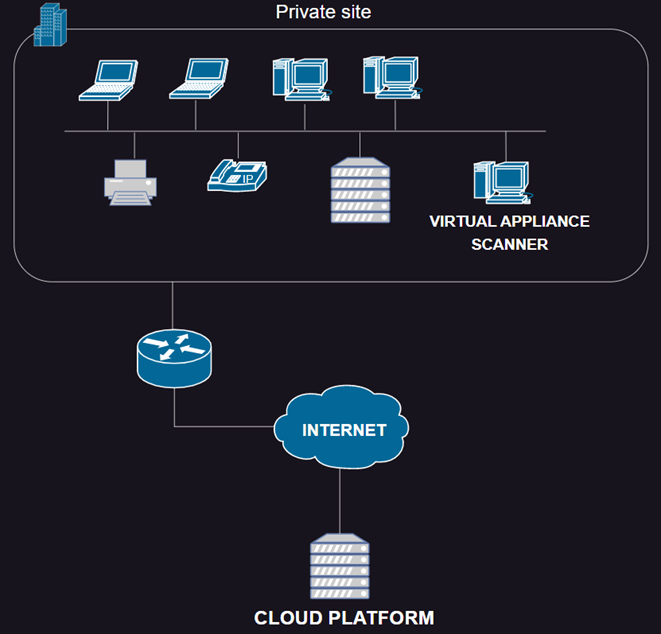
\includegraphics{images/scan_interna.png}
    \caption{: Scansione degli asset interni alla rete.}
    \label{fig:scan_interna}
\end{figure}


Come si evince dall’immagine, la macchina virtuale, oltre ad avere la necessità di accedere alla maggior parte degli asset della rete, ha bisogno di collegarsi a Internet per comunicare con la \textit{cloud platform}. Essa è la piattaforma che gestisce l’intero processo di \textit{vulnerability assessment}, dalla pianificazione e programmazione delle scansioni, alla fase di \textit{remediation} e \textit{patch management}\footnote{Attività periodica di gestione, prioritizzazione, selezione e schedulazione degli aggiornamenti dei software e dei sistemi.}. Una volta installata e configurata la \textit{virtual appliance} è possibile procedere con l’esecuzione della scansione dei \textit{target}.

Il funzionamento di una scansione delle vulnerabilità può essere ridotto al funzionamento di un \textit{port scanner}. Essa infatti esegue una serie di tentativi di connessione con le porte di un sistema, andando quindi a verificare quali servizi sono in ascolto. Poiché un sistema possiede oltre 65.000 porte (precisamente \(2^{16}\)), risulterebbe molto dispendioso in termini di tempo analizzarle tutte. A questo si aggiunge il fatto che un gran numero di queste porte non viene normalmente utilizzato dai sistemi operativi. Ecco perché il tool di scansione considera principalmente le prime 1024 porte, le cosiddette \textit{well-known ports}. Queste includono, ad esempio, le porte 80 e 443, tipiche dei web server, che offrono servizi in HTTP e HTTPS, le porte 22 e 23 che permettono l’accesso remoto al sistema tramite il protocollo sicuro SSH e insicuro Telnet, oppure la porta 21 che identifica il servizio di trasferimento file FTP. Oltre a queste porte è possibile configurare lo scanner in modo che analizzi anche porte specifiche. Se, ad esempio, si vuole verificare l’esposizione di servizi SQL vulnerabili di un database è possibile specificare la porta 3306 per MySQL, oppure la porta 5432 per PostgreSQL.

Una volta identificate le porte in ascolto e stabilita una connessione (nel caso in cui si tratti di porte TCP) lo scanner invia, per ognuna di esse, determinate richieste e comandi. Il comando più semplice che un tool può eseguire è la richiesta del numero di versione del servizio esposto dalla porta in questione. A quel punto il sistema \textit{target} può rispondere alla richiesta normalmente come se il comando fosse eseguito localmente, ad esempio da linea di comando, oppure, se il sistema è configurato a dovere, può rispondere oscurando il riferimento alla versione del servizio. Questo dato può sembrare irrilevante, ma per un ipotetico malintenzionato conoscere la versione dei servizi esposti da un sistema è il primo passo per pianificare l’attacco. Gli \textit{hacker} si muniscono di \textit{toolkit}, ad esempio \textit{metasploit}, che raggruppano insiemi di \textit{exploit} in base alle diverse vulnerabilità note di vari applicativi. Tramite il numero di versione possono quindi identificare, ad esempio con una semplice ricerca in internet, quali vulnerabilità affliggono il servizio in questione. Di conseguenza è possibile risalire relativamente facilmente anche ai rispettivi \textit{exploit} ed eseguire quindi l’attacco.

Si prenda in considerazione lo scenario di un web server Apache pronto a ricevere richieste HTTP o HTTPS. Possiamo collegarci al server con indirizzo IP 172.17.22.233 tramite la porta 80:

\begin{minted}{powershell}
  $ telnet 172.17.22.233 80
\end{minted}

Una volta instaurata la connessione inviamo la seguente richiesta:

\begin{minted}{powershell}
  > HEAD / HTTP/1.0
\end{minted}

E come risposta otteniamo:

\begin{minted}{powershell}
  HTTP/1.1 200 OK
  Date: Fri, 14 Jul 2023 21:23:59 GMT
  Server: Apache/2.4.52 (Ubuntu)
  Last-Modified: Fri, 14 Jul 2023 18:50:47 GMT
  ETag: "29af-60076ed4a731c"
  Accept-Ranges: bytes
  Content-Length: 10671
  Vary: Accept-Encoding
  Connection: close
  Content-Type: text/html
\end{minted}

Come si può notare, in corrispondenza della voce “Server” viene indicata sia la versione del servizio, in questo caso Apache 2.4.52, sia il sistema operativo. Con una semplice modifica al file di configurazione del web server Apache è possibile nascondere questi dati. Ora la risposta alla stessa richiesta è la seguente:

\begin{minted}{powershell}
  HTTP/1.1 200 OK
  Date: Sat, 15 Jul 2023 08:06:19 GMT
  Server: Apache
  Last-Modified: Fri, 14 Jul 2023 18:50:47 GMT
  ETag: "29af-60076ed4a731c"
  Accept-Ranges: bytes
  Content-Length: 10671
  Vary: Accept-Encoding
  Connection: close
  Content-Type: text/html
\end{minted}

Ritornando al funzionamento dello scanner, esso oltre a richiedere generiche informazioni sul servizio, può metterlo alla prova attivamente. Se ad esempio rileva che la porta 139, cioè il servizio NetBIOS\footnote{\textit{Network Basic Input/Output System} è un protocollo obsoleto per le comunicazioni sulla rete locale solitamente attivo in ambienti Windows.}, è in ascolto, può tentare di effettuare una enumerazione dei nomi dei computer e degli utenti appartenenti al dominio aziendale, o delle cartelle di rete condivise. Ad esempio con il seguente comando:

\begin{minted}{powershell}
  $ nbtscan -v 192.168.1.52
\end{minted}

È possibile visualizzare il nome NetBIOS del target e i suoi servizi disponibili:

\begin{minted}{powershell}
  NetBIOS Name Table for Host 192.168.1.52:
  Name          Service          Type
---------------------------------------------------
  MIRO-PC        <20>           UNIQUE
  MIRO-PC        <00>           UNIQUE
  WORKGROUP      <00>           GROUP
  WORKGROUP      <1e>           GROUP
\end{minted}

Il tag 20 identifica il servizio di condivisione risorse di rete. Lo scanner può quindi andare più a fondo e tentare di verificare se nel \textit{target} è attiva la cosiddetta \textit{null session}, che permette ad un utente remoto di accedere a certe risorse del sistema tramite connessioni anonime, quindi senza username e password, ovvero una sessione nulla:

\begin{minted}{powershell}
  $ smbclient //192.168.1.52/IPC$ -U""

  Anonymous login successful
  Try "help" to get a list of possible commands.
  
  smb: \> ls
  NT_STATUS_ACCESS_DENIED listing \*
\end{minted}

Come si può notare è stato possibile accedere anonimamente alla \textit{share} remota, la quale però, in questo caso, permette giustamente un accesso limitato. L’accesso anonimo, inoltre, permette in alcuni casi, ad esempio se il sistema in oggetto fa parte di un dominio, di enumerare gli username di accesso agli account di tale dominio. Una volta che si conoscono i nomi utente basterà un semplice attacco \textit{brute-force} per trovare uno username con associata una password comune.

Lo strumento di scansione, quindi, a seconda della risposta da parte del \textit{target} a una certa richiesta che mira a verificare la presenza o meno di una falla di sicurezza, classifica il servizio esposto come vulnerabile se tale risposta trova una corrispondenza nel database delle vulnerabilità consultabile nella piattaforma in cloud.

Lo scopo di una scansione esterna (Figura \ref{fig:scan_esterna}), invece, è quello di evidenziare le debolezze di un’infrastruttura di rete dal punto di vista di un attaccante posto al di fuori della rete privata aziendale. Si vuole, quindi, valutare la sua sicurezza e la corretta configurazione delle interfacce pubbliche dei dispositivi posti “ai bordi” della rete. Di conseguenza non è possibile giungere a questo obiettivo tramite uno strumento di scansione posto all’interno della rete che si vuole analizzare. La soluzione è utilizzare un \textit{cloud scanner}. Questi strumenti sono programmi in cloud che girano su server esterni di proprietà di aziende specializzate in sicurezza informatica. Nella configurazione di questa tipologia di scansione vengono specificati tutti i possibili \textit{endpoint} della rete in oggetto: gli indirizzi IP delle interfacce pubbliche di firewall e router, eventuali collegamenti a VPN e riferimenti di possibili server esposti in rete, anche in forma di nomi di dominio.

%Di seguito uno schema di tale concetto.

\begin{figure}[h]
\centering
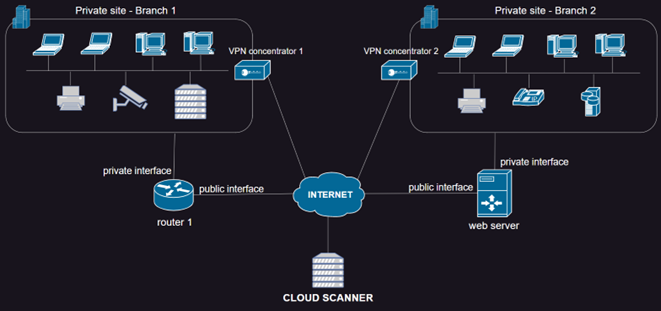
\includegraphics[scale=1.2]{images/scan_esterna.png}
    \caption{: Scansione degli asset ai confini della rete aziendale.}
    \label{fig:scan_esterna}
\end{figure}


Tramite questa architettura la piattaforma esterna in cloud è in grado di interrogare gli apparati di rete sulle loro interfacce pubbliche. Solitamente vengono rilevate configurazioni deboli come l’utilizzo di protocolli di sicurezza obsoleti oppure generiche vulnerabilità di server esposti.

Finora abbiamo preso in considerazione le scansioni \textit{agentless}, ovvero quelle scansioni che vengono eseguite attivamente da uno strumento di analisi, sia esso una \textit{virtual appliance} o un \textit{cloud scanner}. Esistono però anche le scansioni basate sui cosiddetti agenti. Una configurazione \textit{agent-based} consiste nell’avere per ogni \textit{host target} (oppure per i più critici) un software, chiamato agente, installato localmente nella macchina. Questo programma raccoglie in tempo reale i parametri del sistema, l’utilizzo delle risorse, i software installati, le connessioni di rete e gli eventi più sospetti. Oltre a queste informazioni, l’agente, come un qualsiasi software antivirus, effettua periodiche scansioni del sistema sul quale è installato. Un grande vantaggio di questa soluzione consiste nell’avere per ogni asset report più accurati e meno falsi negativi, inoltre le analisi possono essere effettuate in autonomia dalle singole macchine senza compromettere la disponibilità della rete. Ulteriore vantaggio da questa soluzione si ha quando l’azienda permette di ospitare, magari occasionalmente, dispositivi non gestiti, ad esempio i cosiddetti BYOD (\textit{Bring Your Own Device}). Questi dispositivi sono una reale minaccia per la rete aziendale in quanto sono ad uso personale, non sono monitorati e molto spesso contengono software non aggiornati e vulnerabili. Risulta quindi evidente che una valutazione periodica \textit{agentless} dell’infrastruttura non sia ottimale in questo caso. È plausibile infatti che durante tali scansioni non sempre questi dispositivi siano presenti fisicamente nella rete aziendale e che quindi non sia possibile valutarne e correggerne le vulnerabilità. Per questo motivo, in scenari come quello appena illustrato, conviene tenere in considerazione le scansioni basate sugli agenti. Idealmente una scansione per le vulnerabilità dovrebbe consistere in un approccio ibrido: imbastire una scansione \textit{agentless} in modo da valutare lo stato generale della rete, permettendo anche di rilevare e analizzare asset che non erano stati presi in considerazione; predisporre per gli asset più sensibili ed esposti a rischi delle scansioni \textit{agent-based}.

I dati raccolti dalle scansioni vengono poi inviati alla piattaforma in cloud e processati in report.

\section{Analisi dei risultati}
Senza un’accurata ispezione dei risultati, prima di presentarli al committente, il \textit{vulnerability assessment} avrebbe un valore molto limitato.

Al termine delle scansioni lo strumento di analisi genera automaticamente un report per ogni attività, che prende il nome di \textit{technical report}. Questi documenti raccolgono, per ogni \textit{subnet} analizzata, tutte le informazioni e i dati utili rilevati sui singoli dispositivi. Tra questi vi sono, oltre al numero di vulnerabilità suddiviso per criticità e tipologia e le rispettive descrizioni, riferimenti ai sistemi operativi rilevati e ai servizi attivi in ascolto. Tali report, in quanto generati in automatico, necessitano di essere revisionati accuratamente per verificare eventuali inesattezze o imprecisioni. Come in qualsiasi attività di \textit{testing}, infatti, è molto probabile che possano essere presenti falsi positivi. Prendiamo, ad esempio, in considerazione lo scenario in cui un web server venga interrogato dal \textit{vulnerability scanner}. Quest’ultimo, a seconda del \textit{payload} che invia, si aspetta una determinata risposta da parte del server se questo è vulnerabile. Tuttavia, se la risposta è ambigua o non rientra tra gli scenari che il tool di scansione si aspetterebbe, lo scanner potrebbe classificare in modo inesatto il server. Esso, ad una determinata richiesta, potrebbe smettere di rispondere quando al contrario lo scanner si aspetterebbe una risposta, per esempio un messaggio di errore nel caso in cui non fosse vulnerabile. Come interpretare questa assenza di risposta? La \textit{query} dello scanner potrebbe aver causato un’interruzione del servizio e quindi il server sarebbe vulnerabile ad attacchi di tipo \textit{Denial of Service}. Tuttavia, il server potrebbe aver deciso di interrompere la connessione seguendo un meccanismo di difesa implementato ad esempio dall’amministratore di sistema. In questi casi lo strumento di scansione interpreterà l’evento ipotizzando lo scenario peggiore e classificherà il \textit{target} come vulnerabile. È preferibile, infatti, avere falsi positivi rispetto a rischiare di ignorare una possibile vulnerabilità. Altro rumore di fondo ricorrente nei report generati è dovuto alla valutazione della validità dei certificati SSL installati sui dispositivi. Ovviamente è corretto che lo scanner identifichi e controlli la validità di un certificato, quindi che esso risulti emesso da un’autorità attendibile o che non sia scaduto. A nessuna azienda farebbe piacere ricevere segnalazioni dai propri clienti riguardo a problemi di accesso e avvisi di sicurezza del proprio sito web. Diversa invece è la questione quando si tratta di certificati \textit{self-signed} installati in quei dispositivi di gestione come router, firewall, switch, ecc. ai quali si può accedere solo dalla rete locale interna. Questi dispositivi possiedono un certificato auto generato ma, dato che solitamente l’accesso a tali dispositivi viene effettuato direttamente tramite indirizzo IP privato, l’errore che il browser propone può essere ignorato, in quanto siamo consapevoli che stiamo contattando il dispositivo con quello specifico indirizzo. Inoltre non vi è nemmeno il rischio di intercettazione di informazioni in chiaro, in quanto se il dispositivo possiede un certificato correttamente installato ed è configurato per rispondere in HTTPS, la connessione verrà crittografata pur trattandosi di un certificato non riconosciuto. Data la quantità di dispositivi di gestione presenti in una rete aziendale, si può immaginare quanto “rumore” essi possano causare in un \textit{technical report}. È per questo che è importante usare i risultati delle prime scansioni per affinare e calibrare lo strumento aggiungendo nella sua configurazione eventuali eccezioni. Nel seguito questo aspetto verrà illustrato più in dettaglio.

Il lavoro dell’analista è quindi quello di interpretare, nel modo più oggettivo possibile, i risultati ottenuti riportandoli in un \textit{executive report}, il documento che verrà presentato al cliente. L’analista, oltre a dover discernere ciò che è irrilevante e fuorviante da ciò che necessita realmente di attenzione, deve contestualizzare i risultati restando il più possibile attinente alle informazioni oggettive ottenute dal \textit{technical report}. Il documento, infatti, verrà consultato anche dall’eventuale reparto IT dell’azienda cliente. Dato che solo loro possiedono il preciso quadro generale della propria infrastruttura, sbilanciarsi con certe supposizioni riguardo ad esempio una composizione non ottimale della rete, oppure l’identificazione di una precisa tipologia di dispositivo, rischia di invalidare il lavoro svolto portando a delle conclusioni false e a una cattiva reputazione agli occhi dell’azienda cliente. Non bisogna dimenticare che, a meno di specifiche configurazioni, lo scanner di rete non ha alcuna conoscenza riguardo l’infrastruttura in questione e ogni informazione che rileva in merito alle vulnerabilità è basata esclusivamente dalle corrispondenze che individua tra le risposte dei \textit{target} e quelle contenute in un database limitato.

I risultati delle analisi dovranno essere esposti anche al personale amministrativo. L’analista deve riportare i risultati nell’\textit{executive report} in linguaggio naturale limitando i termini tecnici. Il documento dovrà quindi essere comprensibile da persone non esperte e illustrerà, anche per mezzo di grafici, per ogni \textit{subnet} analizzata, la relativa situazione in termini di numero, criticità e distribuzione delle vulnerabilità. Insieme a una breve descrizione delle criticità più rilevanti, ne verranno date delle possibili soluzioni.

\section{Remediation}

Un’esecuzione periodica del \textit{vulnerability assessment} permette di identificare prima di un potenziale malintenzionato le criticità maggiori all’interno e all’esterno della rete aziendale. La fase di risoluzione di tali criticità è un altrettanto regolare processo di indagine e documentazione degli asset vulnerabili più esposti. Il documento riepilogativo, stilato nella fase di analisi dei risultati, permette ai tecnici e ai manager di avere una visione di insieme riguardo gli asset e le sottoreti più a rischio e considerare quindi le migliori soluzioni, anche a lungo termine. Al termine di ogni descrizione delle risultanze trovate nei \textit{target} viene presentata una loro possibile risoluzione. Nell’\textit{executive report} questa consiste in una spiegazione sintetica, mentre il \textit{technical report} dato in mano al reparto IT aziendale presenta le problematiche e le relative risoluzioni in modo più specifico e pratico, con riferimenti alla documentazione ufficiale dei servizi in uso.

Le vulnerabilità sono classificate in base alla loro severità, seguendo una serie di metriche che verranno presentate nel seguito. Vulnerabilità con \textit{severity} bassa e media non presentano un rischio diretto per la sicurezza dell’infrastruttura aziendale, ma se sfruttate potrebbero rivelare informazioni utili a un potenziale attaccante per la pianificazione ed esecuzione di un attacco. Le vulnerabilità di livello alto e critico invece necessitano di interventi tempestivi in quanto il loro \textit{exploit} permette gravi compromissioni alla confidenzialità, integrità o disponibilità della rete.

Idealmente la fase di \textit{remediation} dovrebbe porre rimedio a tutte quelle vulnerabilità che presentano un livello di rischio considerevole. Nel seguito verranno presentate le tipologie di vulnerabilità che richiedono maggiore attenzione. Nella pratica, eliminare e isolare più falle possibili richiede un’accurata analisi dei sistemi attivi, dei rispettivi servizi esposti sia verso la rete pubblica che nella intranet aziendale e delle politiche di visibilità e connessione tra le varie \textit{subnet} aziendali.

Porre rimedio alle debolezze trovate durante l’analisi vuol dire anche trovare dei compromessi fra la praticità e la comodità di utilizzo dei sistemi con i quali ci si interfaccia e la loro conformità dal punto di vista della sicurezza. Si pensi ad esempio all’implementazione di meccanismi di autenticazione a doppio fattore\footnote{Meccanismo che in fase di autenticazione a un servizio richiede, oltre a username e password, l'inserimento di un codice temporaneo generato da un proprio dispositivo mobile in modo da dimostrare il suo possesso.} o all’introduzione di politiche più stringenti in merito ai comportamenti ai quali gli utenti finali devono attenersi. Altri compromessi possono riguardare cali di \textit{performance} della rete a seguito dell’installazione di dispositivi e/o software di analisi e scansione dei pacchetti di rete delle connessioni in entrata e in uscita \cite{remediation}.

Per tenere traccia dei progressi, in termini di risoluzione delle problematiche, vengono stilati i \textit{vulnerability assessment} 
comparativi. Questi documenti prendono in considerazione due o più periodi nei quali si è svolta una valutazione della sicurezza e li compara con i risultati dell’ultima esecuzione di un \textit{vulnerability assessment}. Questo permette di avere uno storico dettagliato con quantità e tipologia di vulnerabilità e di dispositivi affetti potendo metterlo in relazione con la rilevazione più recente e valutando quindi l’operato e gli sforzi dell’azienda nella messa in sicurezza degli \textit{asset} più esposti e vulnerabili.

Infine, al termine di ogni ciclo di \textit{remediation}, tutti i documenti redatti, ad eccezione dei \textit{technical report}, vengono discussi insieme al committente e al responsabile del reparto IT.


\chapter{Caso di studio: analisi delle vulnerabilità di una rete aziendale} \label{cap:part-2}
In questo capitolo si espone un caso di studio reale di \textit{vulnerability assessment} eseguito per un'azienda metalmeccanica che produce componenti per il settore dell'Automotive.

La scansione è stata eseguita tra gennaio e febbraio 2023 e fa parte della commessa richiesta dall'azienda per la valutazione della sicurezza della propria rete, che prevede, oltre al \textit{vulnerability assessment}, attività di \textit{penetration test} e campagne di \textit{phishing}\footnote{Attacchi di \textit{phishing} simulati, per email o SMS, che permettono all'azienda di conoscere il livello di consapevolezza dei propri dipendenti in materia di sicurezza informatica.}.

\section{Metriche} \label{metriche}
Le vulnerabilità di un sistema informatico sono classificate in base alla loro gravità, e quindi al pericolo che esse possono comportare a tale sistema, in modo da poter prioritizzare gli interventi di risoluzione.

Il livello di \textit{severity} è calcolato principalmente secondo le seguenti metriche e viene espresso attraverso il CVSS \textit{score}\footnote{Il \textit{Common Vulnerability Scoring System}, originariamente sviluppato dal \textit{National Infrastructure Advisory Council}, è un sistema standardizzato che assegna un punteggio da zero a dieci (severità più alta) alle vulnerabilità.}.

\paragraph{Vettore di attacco (AV)} Determina il minimo livello di prossimità (sia logica che fisica) che permette a un attaccante di eseguire l'\textit{exploit} della vulnerabilità. I livelli, ordinati per valore decrescente, sono:

    \begin{itemize}
        \item \textit{Network.} È possibile eseguire l'attacco al livello di Rete dello \textit{stack} ISO/OSI, quindi anche attraverso Internet. Un esempio è un attacco \textit{Denial of Service} eseguito aprendo una serie di connessioni TCP su un indirizzo IP pubblico remoto.
        \item \textit{Adjacent.} Per eseguire l'attacco è necessario risiedere nello stesso segmento di rete del dispositivo vulnerabile. Si noti che non è necessario essere vicini fisicamente al \textit{target}. Un'azienda può avere più sedi e condividere le stesse \textit{subnet} attraverso ponti radio o collegamenti VPN.
        \item \textit{Local.} La vulnerabilità non può essere sfruttata attraverso la rete. L'attaccante ha bisogno di accedere fisicamente al \textit{target} oppure deve indurre l'utente ad eseguire specifiche azioni su di esso mediante, ad esempio, tecniche di \textit{social engineering}.
        \item \textit{Physical.} A questo livello l'attaccante deve avere accesso fisico, anche costante, alla macchina vulnerabile. Per sfruttare la vulnerabilità deve manomettere fisicamente il \textit{target}, ad esempio tramite il collegamento di un'unità USB esterna che permette di compromettere il sistema e dare l'accesso all'attaccante.
    \end{itemize}

\paragraph{Complessità dell'attacco (AC)} Come si evince dal nome, questa metrica indica il livello di difficoltà di \textit{exploit} della vulnerabilità, ossia le condizioni, fuori dal controllo dell'attaccante, che devono esistere per portare a termine l'attacco.

    \begin{itemize}
        \item \textit{Low.} L'attacco può essere eseguito con successo ripetutamente senza bisogno di condizioni specifiche.
        \item \textit{High.} L'attacco ha successo solo dopo un'estesa preparazione e indagine della macchina \textit{target} e del relativo ambiente. L'attacco potrebbe implicare grosse computazioni e numerosi tentativi prima di giungere a un successo.
    \end{itemize}

\paragraph{Privilegi richiesti (PR)} Questa metrica indica il livello di privilegi, all'interno dell'ambiente vulnerabile, necessari all'attaccante affinché possa eseguire l'\textit{exploit} della vulnerabilità.

    \begin{itemize}
        \item \textit{None.} L'attaccante non ha bisogno di alcun privilegio per portare a termine l'attacco. Non ha bisogno di accedere né a configurazioni, né a file di sistema.
        \item \textit{Low.} L'attaccante ha bisogno dei privilegi di un utente base del sistema.
        \item \textit{High.} L'attaccante ha bisogno di permessi amministrativi per poter modificare configurazioni critiche e file di sistema.
    \end{itemize}

\paragraph{Interazione dell'utente (UI)} Indica se la vulnerabilità in oggetto, per essere sfruttata, ha bisogno della collaborazione (involontaria) di un altro utente.

    \begin{itemize}
        \item \textit{None.} Il sistema può essere compromesso dall'attaccante senza l'intervento di terzi.
        \item \textit{Required.} È necessaria l'interazione di un utente. Ad esempio l'installazione di un \textit{Trojan} nel sistema affetto dalla vulnerabilità.
    \end{itemize}

\paragraph{Scope (S)} Questa metrica indica se l'\textit{exploit} della singola vulnerabilità che affligge un sistema, ad esempio un'applicazione, un sistema operativo o un dispositivo di rete, impatta anche su altri sistemi esterni ad esso.

    \begin{itemize}
        \item \textit{Changed.} L'attacco permette di compromettere anche risorse che risiedono in un ambito diverso da quello del sistema vulnerabile. Ad esempio la vulnerabilità di un'applicazione che permette all'attaccante di prendere il controllo del sistema operativo come amministratore.
        \item \textit{Unchanged.} L'attacco impatta solo sul sistema vulnerabile.
    \end{itemize}

\paragraph{} Infine vi sono le metriche relative alla triade CIA, che misurano l'impatto di un attacco, causato dalla vulnerabilità in oggetto, sulla \textbf{Confidenzialità (C)}, \textbf{Integrità (I)} e \textbf{Disponibilità (A)} delle risorse del sistema violato.
Anche in questo caso i valori delle metriche sono definiti in \textit{High}, \textit{Low} e \textit{None}.

\paragraph{} Il CVSS non è l'unico \textit{scoring system} esistente ma offre un \textit{framework} su cui basarsi. Diversi \textit{vendor} classificano le vulnerabilità dei propri sistemi o, nel caso degli scanner di rete, le vulnerabilità rilevate sui \textit{target} della scansione, in modo diverso avendo comunque come metriche di base quelle appena esposte.

\section{Strumentazione}
Esistono un gran numero di \textit{vulnerability scanning tools} che differiscono, oltre che per il prezzo, in base alle tecnologie che supportano (oltre a Windows, Linux e macOS potrebbero esserci sistemi insoliti per i quali lo scanner non è stato programmato), se sono dedicati anche alle \textit{web applications scans} e in base ad eventuali configurazioni come il grado di automazione e la possibilità di schedulare le scansioni. La maggior parte dei tool di scansione però consiste in software accessibili da piattaforme in cloud attraverso il browser.

Nel caso in oggetto si è impiegato lo strumento Qualys VMDR (Vulnerability Management, Detection, and Response). Nell'appendice \ref{appendix:a} viene illustrato come si presenta il software.

Tramite la sua interfaccia è possibile avere una panoramica delle scansioni già eseguite, in esecuzione o programmate e delle vulnerabilità trovate più di frequente, è possibile consultare i \textit{technical} ed \textit{executive} report e creare dei piani di \textit{remediation}. Fondamentale è anche la possibilità di consultare il database costantemente aggiornato delle ultime vulnerabilità pubblicate.

È possibile inoltre organizzare gli asset in gruppi che andranno a definire i \textit{target} della scansione (Figura \ref{fig:qualys_targets}).

Qualys assegna un punteggio alle vulnerabilità da uno a cinque e consiste il più delle volte in una normalizzazione del punteggio ottenuto dal CVSS.

\section{\textit{Target definition}}
Lo \textit{scope} della scansione viene definito dal cliente e, insieme al reparto IT, vengono comunicate tutte le \textit{subnet} da includere, o le più prioritarie. Questo VA considera 27 sottoreti private distinte e 4 indirizzi IP pubblici. Le figure \ref{fig:target_definition_int} e \ref{fig:target_definition_ext} illustrano una porzione del documento che specifica tali indirizzi. Le prime quattro lettere di ogni \textit{target} identificano il cliente.

\begin{figure}[h]
\centering
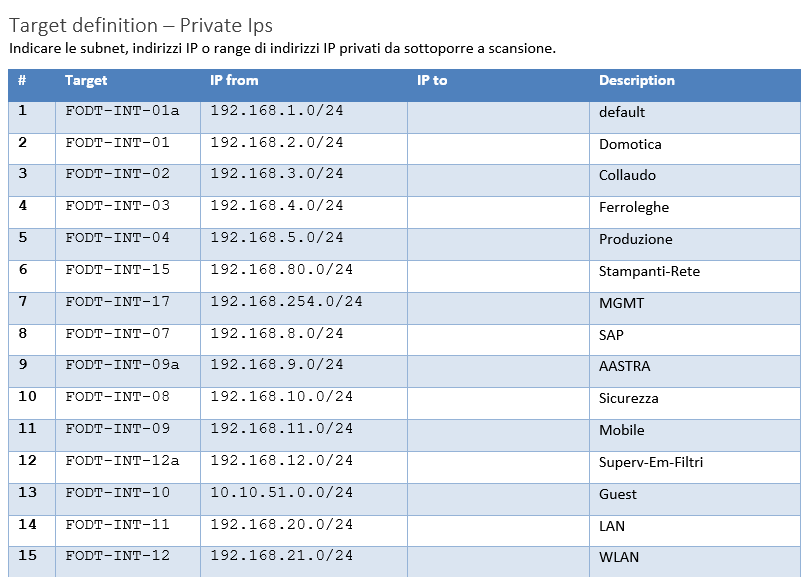
\includegraphics[scale=0.8]{images/target_definition_int.png}
    \caption{: Definizione dei \textit{target} privati.}
    \label{fig:target_definition_int}
\end{figure}

Come si può notare dalla figura \ref{fig:target_definition_int}, oltre alla definizione delle reti oggetto della scansione, viene data anche una loro descrizione in merito al loro ambito. Questo dato, se non viene indicato dai sistemisti dell'azienda, può essere estrapolato eseguendo una preliminare \textit{discovery scan} in modo da rilevare i sistemi operativi e i servizi attivi. In questo caso però i risultati sono indicativi e potrebbero quindi portare a imprecisioni.

Stando a quanto dichiarato da questo documento preliminare, l'infrastruttura in questione presenta un buon livello di segmentazione della rete: la rete Guest è su una classe di IP completamente diversa dalle altre, i macchinari di produzione sono separati dalla domotica e anche le stampanti risiedono in una \textit{subnet} diversa da quella delle postazioni di lavoro (LAN). Anche la rete di \textit{management}\footnote{Rete usata dagli amministratori di sistema per accedere ai sistemi di gestione dell'intera infrastruttura, ad esempio host di virtualizzazione, switch, firewall o NAS.} si trova su una rete a sè. Inoltre si nota che la rete wireless (WLAN) è separata dalla LAN cablata.

Queste informazioni sono utili per rendere le scansioni più accurate e per avere un contesto, seppur superficiale, della situazione.

\begin{figure}[h]
\centering
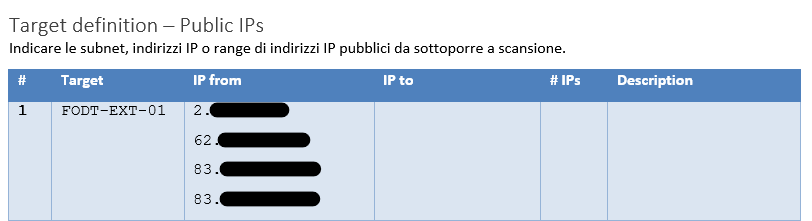
\includegraphics[scale=0.8]{images/target_definition_ext.png}
    \caption{: Definizione dei \textit{target} pubblici.}
    \label{fig:target_definition_ext}
\end{figure}

\section{Configurazione della scansione}
\paragraph{Scansione interna} Prima ancora di configurare e schedulare le scansioni c'è bisogno di fare il \textit{deploy} della \textit{virtual appliance}, ovvero quella macchina virtuale che sarà installata nell'ambiente aziendale e avrà accesso a tutti i \textit{target} in modo da poter comunicare con loro. Nel nostro scenario la macchina virtuale risiederà nella rete 192.168.1.0/24 con un indirizzo IP configurato staticamente (Figura \ref{fig:qualys_appliance}).

A questo punto è necessario configurare le opportune regole di firewall per fare in modo che la macchina virtuale comunichi, tramite tutte le porte o quelle che verranno specificate in seguito, con i segmenti di rete definiti precedentemente. Per fare questo si potrebbe semplicemente creare una regola che permetta il traffico proveniente dalla rete 192.168.1.0/24 verso tutte le altre. Tuttavia, ciò rappresenterebbe una falla di sicurezza da non sottovalutare. Qualsiasi host collegato a tale rete, infatti, sarebbe in grado di comunicare col resto dell'infrastruttura. Certamente questa configurazione sarebbe attiva solamente per il periodo della scansione. Tuttavia le conseguenze che potrebbe portare una dimenticanza da parte dei responsabili nella dismissione di questa regola sarebbero potenzialmente catastrofiche\footnote{Si consideri un \textit{ransomware} che si replica sui segmenti di rete raggiungibili fino a infettare le infrastrutture di backup.}.

La procedura corretta, invece, consiste nel creare una \textit{reservation}\footnote{Prenotazione e assegnazione manuale di un indirizzo IP dal \textit{pool} DHCP a un MAC \textit{address}.} dell'indirizzo IP della macchina e configurare quindi una regola che permetta esclusivamente a quell'indirizzo di contattare le altre sottoreti.

Ora è possibile procedere con la configurazione delle scansioni, una per ogni \textit{target}. Nel caso in questione le scansioni non saranno autenticate (sia per quanto riguarda le utenze di dominio sia per servizi, come gestori di database o di sistemi di virtualizzazione) e analizzeranno circa 1900 porte TCP e circa 180 porte UDP. Inoltre, invece di instaurare un \textit{handshake} TCP completo, eseguiranno una scansione silente\footnote{Lo scanner, una volta ricevuto dal \textit{target} il pacchetto TCP SYN-ACK dopo aver trasmesso SYN, non chiude la procedura di \textit{handshake} a tre vie inviando ACK. Al contrario risponde con un pacchetto RST che chiude la connessione. Questo è utile per identificare le porte aperte del \textit{target} evitando di farsi rilevare da eventuali sistemi di sicurezza.}. La figura \ref{fig:qualys_scan-profile} illustra più nel dettaglio questo profilo di configurazione.

\paragraph{Scansione esterna} Per quanto riguarda la scansione delle interfacce pubbliche dei dispositivi posti ai confini della rete aziendale, la questione della configurazione della \textit{virtual appliance} e la conseguente modifica delle regole di firewall non si pone. La scansione infatti verrà eseguita direttamente dal servizio in cloud. Come si nota dalla figura \ref{fig:qualys_scan_ext} la scansione esterna in questione è stata effettuata dal server di proprietà di Qualys con indirizzo pubblico 64.39.106.5. Il profilo di scansione utilizzato è lo stesso delle scansioni interne.


\begin{figure}[t]
\centering
    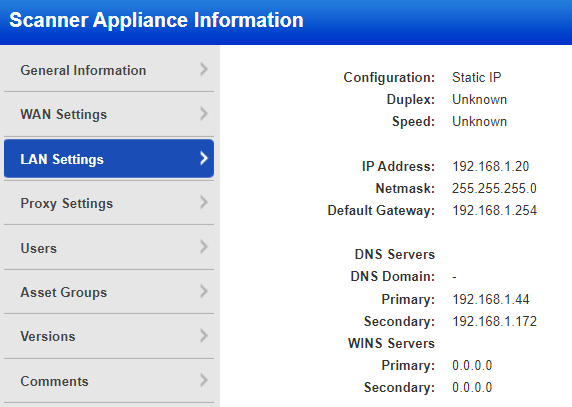
\includegraphics[scale=0.7]{images/qualys_appliance2.png}
    \caption{: Configurazione LAN della \textit{virtual appliance}.}
    \label{fig:qualys_appliance}
\end{figure}

\begin{figure}[t]
\centering
    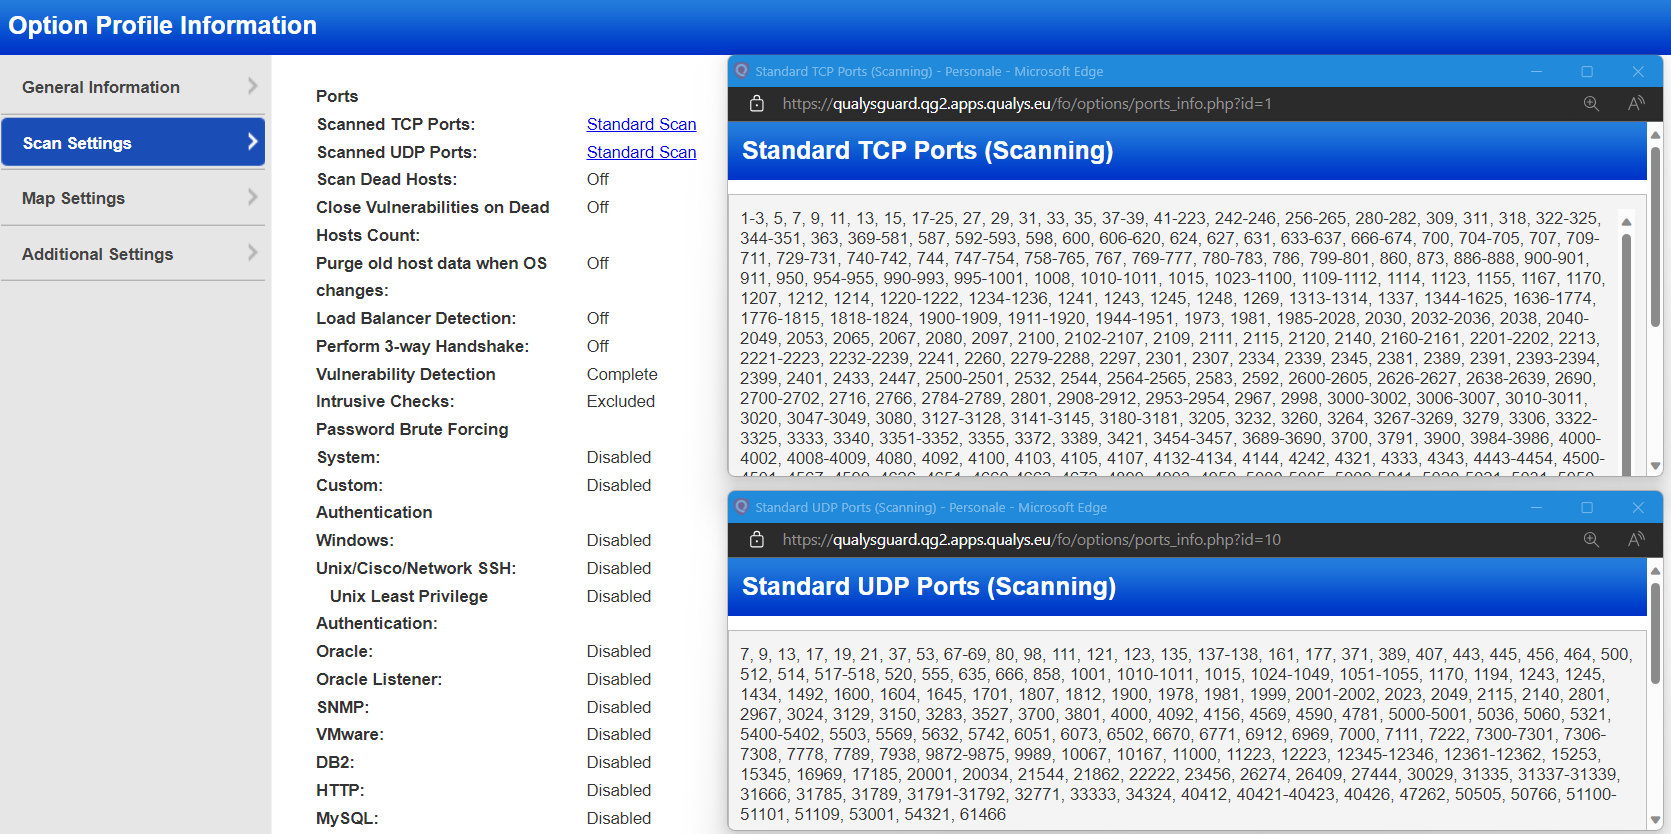
\includegraphics[scale=0.35]{images/qualys_scan-profile.png}
    \caption{: Configurazione del profilo di scansione.}
    \label{fig:qualys_scan-profile}
\end{figure}

\begin{figure}[t]
\centering
    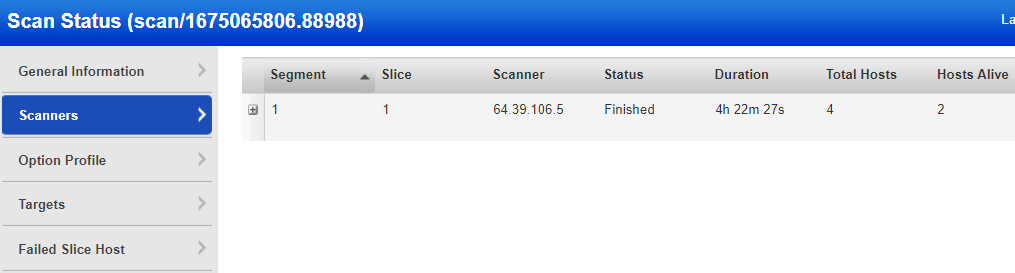
\includegraphics[scale=0.6]{images/qualys_scan_ext.png}
    \caption{: Scansione esterna.}
    \label{fig:qualys_scan_ext}
\end{figure}


\section{Analisi dei report}
Come spiegato nel capitolo precedente, il \textit{tool} di scansione, al termine dell'attività, genera in automatico un \textit{technical report} per ogni \textit{target} analizzato.

Verranno presentati ora i report più significativi ottenuti da questa attività di \textit{assessment}.\newline

\subsection{Target FODT-EXT-01} \textbf{\textit{Figura \ref{fig:fodt-ext-01_1}}}


\begin{figure}[t]
    \centering
    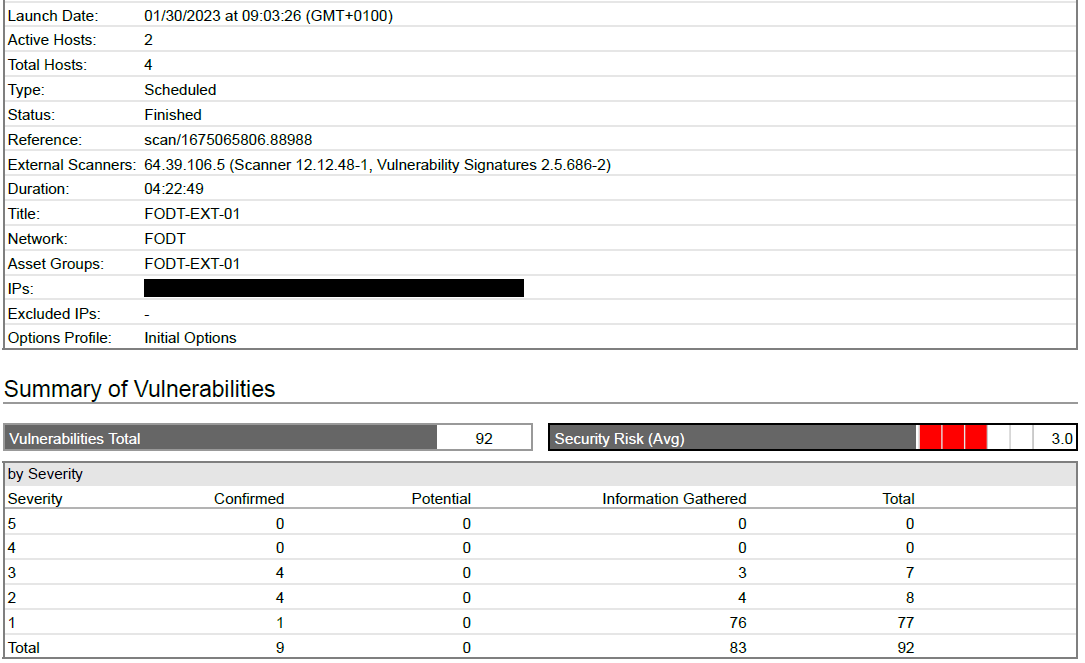
\includegraphics[width=1\linewidth]{images/FODT-EXT-01_1.png}
    \caption{}
    \label{fig:fodt-ext-01_1}
\end{figure}


\begin{figure}[t]
    \centering
    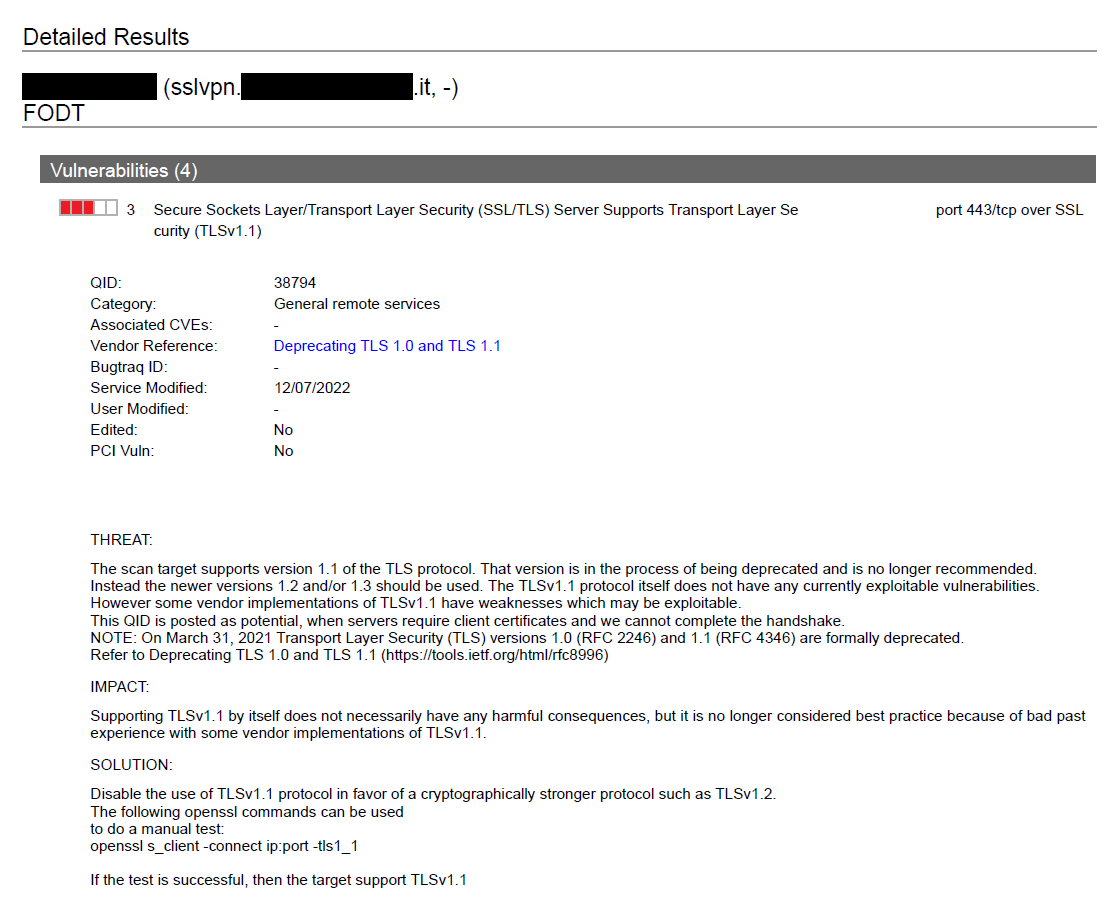
\includegraphics[width=1\linewidth]{images/FODT-EXT-01_2.png}
    \caption{}
    \label{fig:fodt-ext-01_2}
\end{figure}


Su un totale di quattro host, sono state rilevate 92 vulnerabilità sui due host attivi. Il numero di vulnerabilità può sembrare alto, tuttavia in questo numero Qualys include anche le \textit{Information gathered} (che in questo caso sono 83), ovvero tutte le informazioni generiche visibili che il \textit{tool} è riuscito a ricavare dagli apparati da un'analisi superficiale, ad esempio i servizi attivi. Dato che queste informazioni non corrispondono a vere e proprie vulnerabilità in queste analisi verranno prese in considerazione solamente le vulnerabilità categorizzate come \textit{Confirmed}.

In questo caso vi sono quattro vulnerabilità di livello di severità tre e di livello due e una di livello uno. Non sono state rilevate vulnerabilità gravi.
\\ Entrambi gli host, probabilmente due firewall di due connettività diverse, presentano vulnerabilità riguardanti protocolli di crittografia e comunicazione sicura a livello di trasporto SSL/TLS. In particolare il protocollo TLS nella versione 1.0 e 1.1 è obsoleto e formalmente deprecato dal 31 marzo 2021\footnote{RFC 8996.}. Lo scanner ha rilevato che i due host supportano l'utilizzo di tali protocolli.

Le debolezze più grandi di TLS v1.0 e v1.1 risiedono nel fatto che per garantire autenticazione, confidenzialità e integrità delle comunicazioni client-server, si affidano ad algoritmi crittografici e di \textit{hashing} obsoleti e insicuri, come DES e SHA-1\footnote{L'algoritmo crittografico DES (\textit{Data Encryption Standard}) è stato sostituito dal più robusto AES (\textit{Advanced Encryption Standard}).
\\ L'algoritmo di \textit{hashing} SHA-1 è stato oggetto di numerosi studi di crittoanalisti e nel 2011 il NIST lo ha dichiarato deprecato.}.

Per evitare dunque l'utilizzo, anche involontario, di essi è necessario disabilitarli e affidarsi esclusivamente alle implementazioni più recenti TLS v1.2 o v1.3.

La figura \ref{fig:fodt-ext-01_2} mostra i dettagli del risultato di tale rilevazione.
\\ Dal nome DNS rilevato si può notare come uno degli host analizzati sia probabilmente un \textit{gateway} VPN che riceve le connessioni dai client sulla sua interfaccia pubblica attraverso Internet. 
\\ Nel report viene poi presentata una descrizione della vulnerabilità e delle falle di sicurezza che comporta, una descrizione dell'impatto sul sistema nel caso di un eventuale \textit{exploit} della vulnerabilità e le possibili soluzioni.

\subsection{Target FODT-INT-01} \textbf{\textit{Figura \ref{fig:fodt-int-01_1}}} \label{fodt-int-01}


\begin{figure}[t]
    \centering
    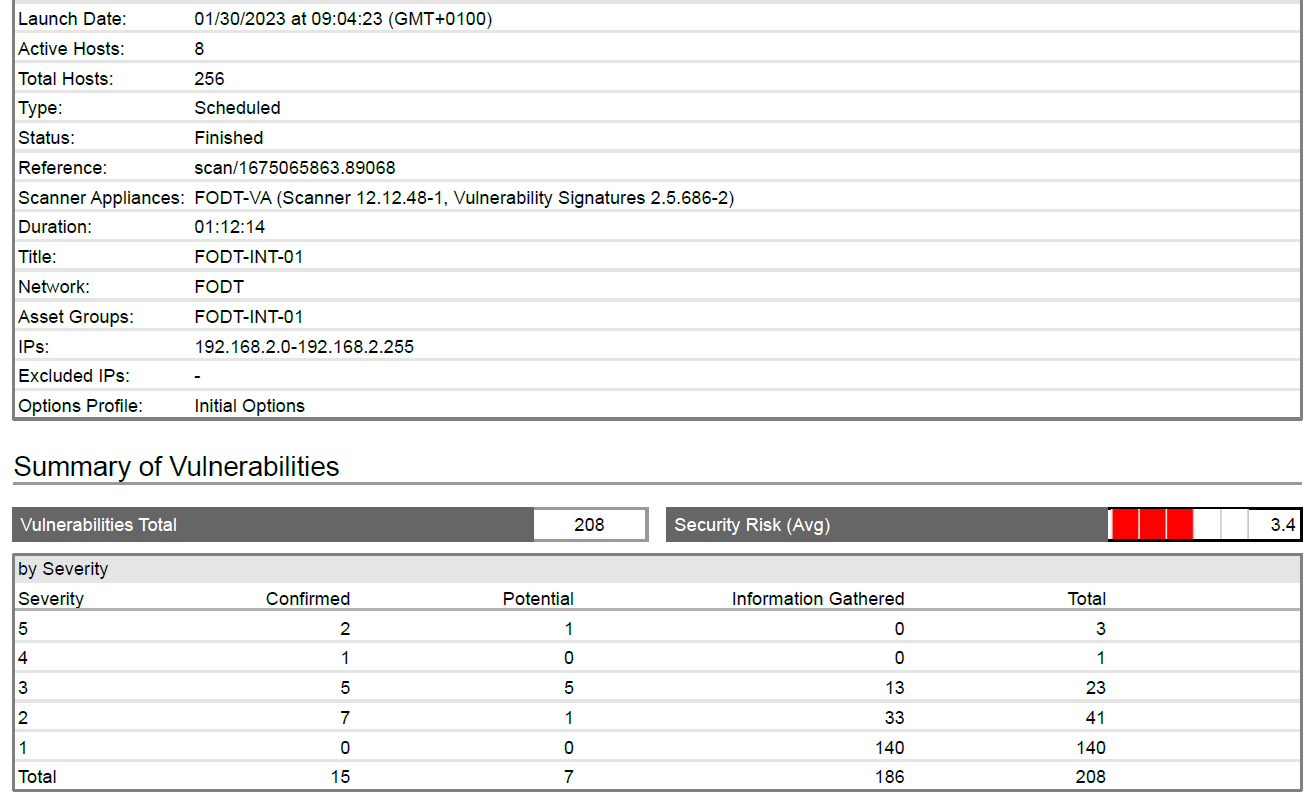
\includegraphics[width=1\linewidth]{images/FODT-INT-01_1.png}
    \caption{}
    \label{fig:fodt-int-01_1}
\end{figure}


\begin{figure}[t]
    \centering
    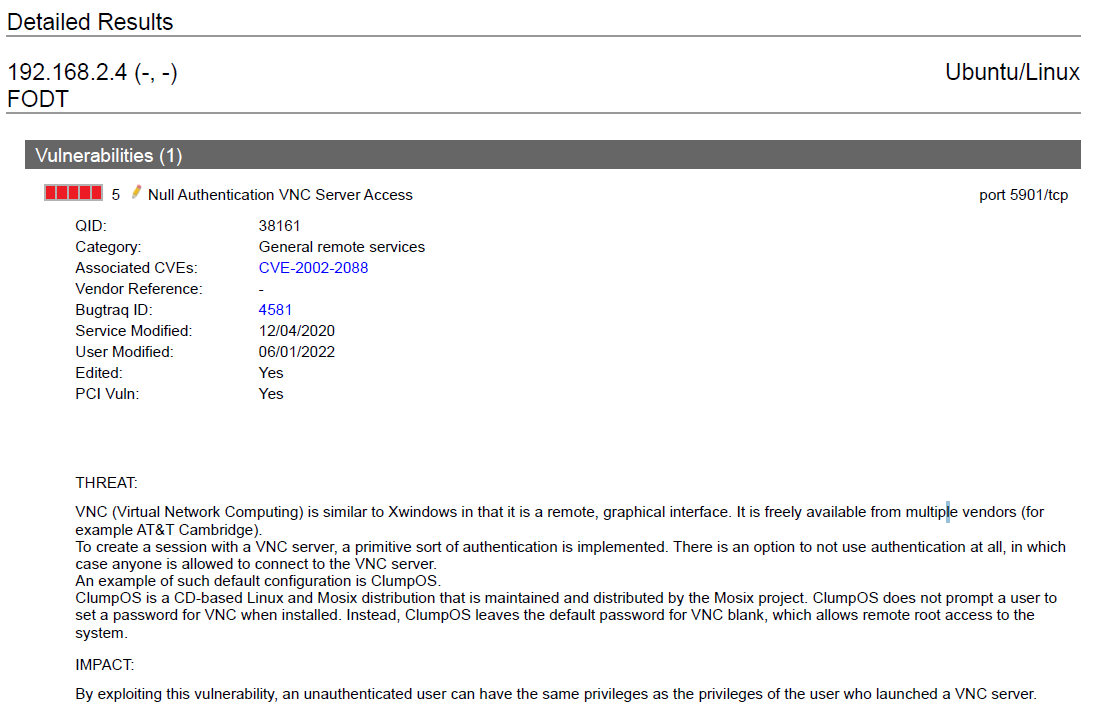
\includegraphics[width=1\linewidth]{images/FODT-INT-01_2.png}
    \caption{}
    \label{fig:fodt-int-01_2}
\end{figure}


Tra i 254 possibili host di questa rete ne sono risultati attivi 8.
Le due vulnerabilità più gravi sono state rilevate negli host 192.168.2.4 e 192.168.2.6. Questi host espongono un servizio di accesso remoto con una configurazione insicura. Il servizio in questione è il VNC (\textit{Virtual Network Computing}). Questo applicativo è costituito da una componente server, installata sul computer remoto che si vuole gestire, e una client, che risiede sui dispositivi che hanno bisogno di accedere all'host remoto. Se il servizio è configurato, come in questo caso, in modo da permettere accessi non autenticati, è possibile, per qualsiasi utente che riesca a collegarsi, accedere al computer "server" senza bisogno di credenziali (Figura \ref{fig:fodt-int-01_2}).
\\ L’host 192.168.2.254 (probabilmente un router o switch) presenta la maggior parte delle vulnerabilità trovate in questo target. In particolare viene segnalata l’esposizione di servizi di connessione remota SSH (\textit{Secure Shell}) in versione obsoleta e Telnet. Entrambi i protocolli permettono di collegarsi e interagire con un host remoto mediante linea di comando con la sostanziale differenza che Telnet non implementa la cifratura della connessione\footnote{Telnet fu sviluppato originariamente tra gli anni '70 e '80 per essere utilizzato in reti fidate governative e istituzionali}. Nel caso in cui l'host in questione fosse un apparato di rete e un amministratore di sistema volesse accedervi, sarebbe possibile per una persona terza, appartenente alla stessa rete, intercettare, ad esempio tramite un attacco ARP \textit{poisoning}\footnote{Una figura terza, che risiede nella stessa sottorete, maschera l'indirizzo MAC del gateway col proprio indirizzo fisico. In questo modo le connessioni con l'esterno o con altre sottoreti passeranno per il falso gateway così da poter essere intercettate e "sniffate".}, la connessione e vedere in chiaro le credenziali di accesso. A causa di questa intrinseca debolezza di Telnet, si predilige l'uso del protocollo SSH.
\\ \textit{Secure Shell} implementa meccanismi di autenticazione e crittografia della connessione client-server. SSH offre la possibilità di autenticare il client e il server attraverso chiavi asimmetriche\footnote{Nell'host client viene generata una coppia di chiavi pubblica e privata generalmente di lunghezza a 2048 o 4096 bit, quindi molto più lunghe di una password convenzionale. La chiave pubblica viene caricata sul server al quale si vuole accedere e, al momento dell'instaurazione della connessione, il server "sfida" il client a decifrare una stringa generata casualmente e cifrata con la chiave pubblica del client. Se come risposta il server riceve la stessa stringa il client è autenticato.}. Questo metodo di autenticazione è alternativo alla classica richiesta di username e password. Di conseguenza permette di evitare i rischi causati dalla configurazione, da parte degli utenti, di password deboli e facili da violare mediante attacchi \textit{brute force}. Una volta instaurata una connessione sicura, client e server si scambiano una chiave di sessione simmetrica per crittografare il traffico.
\\ Nonostante questi meccanismi di sicurezza, SSH nella sua prima versione è risultato vulnerabile ad attacchi \textit{Man-in-the-Middle} (CVE-2001-1473) e \textit{Remote code execution} (CVE-2001-0144). È possibile quindi per un attaccante sia impersonificare il server SSH (o il client) sia indurre da remoto l'esecuzione in locale di codice arbitrario. 


La \textit{remediation} consiste nel considerare la necessità di esporre questi servizi sensibili e nel caso non fossero strettamente necessari di disabilitarli. Si proceda anche con l’aggiornamento o la dismissione, in favore di versioni più recenti (ad esempio SSH-2), dei servizi obsoleti.

\subsection{Target FODT-INT-01A} \textbf{\textit{Figura \ref{fig:fodt-int-01a_1}}}

\begin{figure}[t]
    \centering
    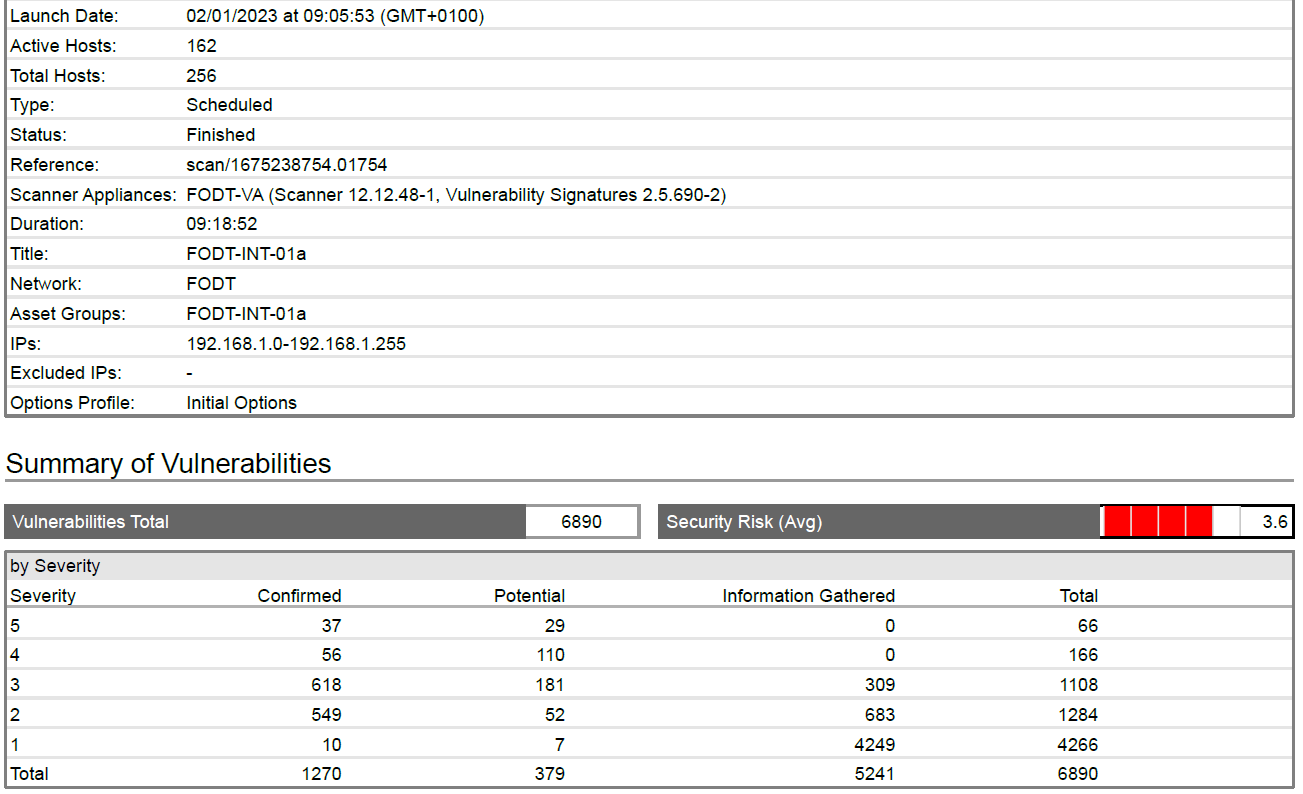
\includegraphics[width=1\linewidth]{images/FODT-INT-01a_1.png}
    \caption{}
    \label{fig:fodt-int-01a_1}
\end{figure}


\begin{figure}[t]
    \centering
    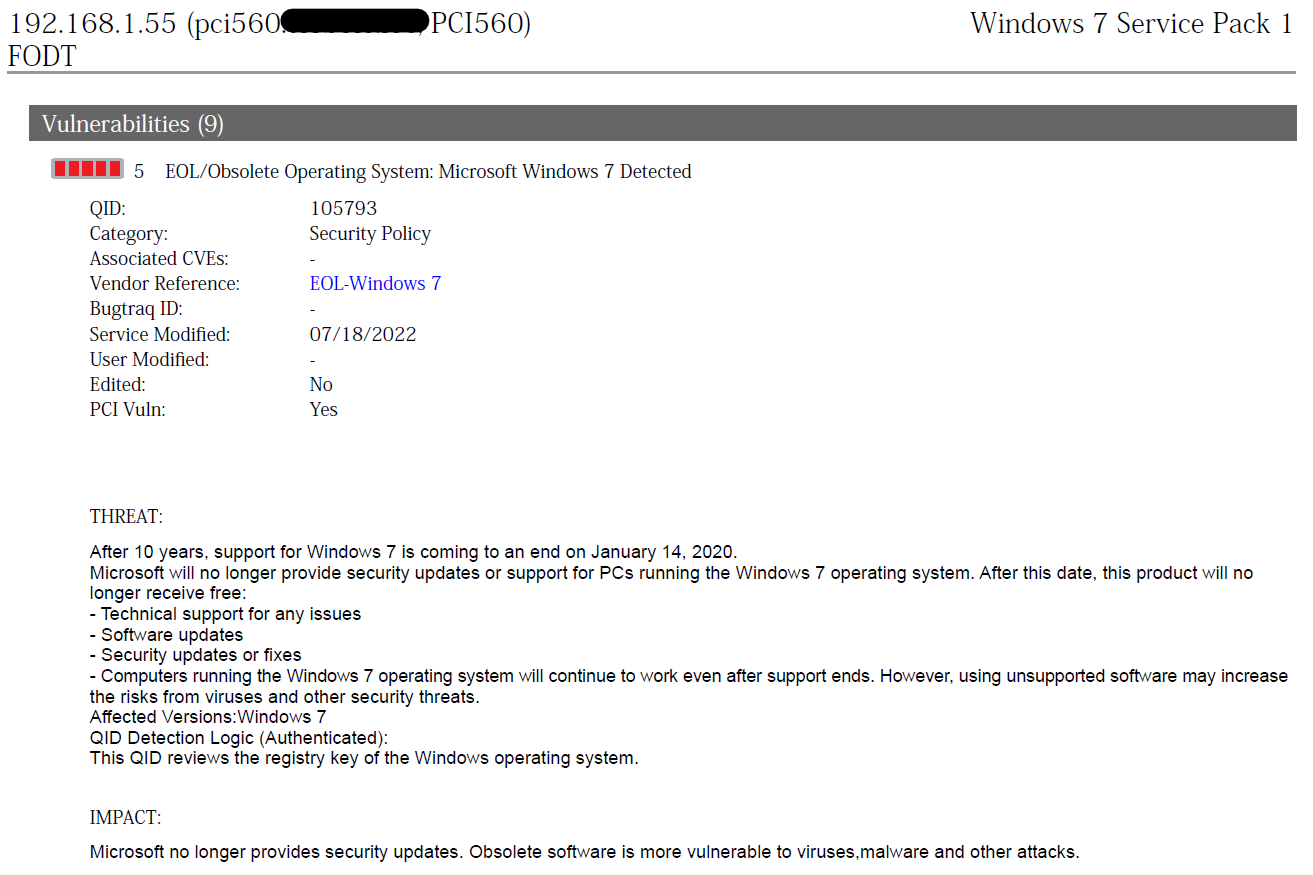
\includegraphics[width=1\linewidth]{images/FODT-INT-01a_2.png}
    \caption{}
    \label{fig:fodt-int-01a_2}
\end{figure}


L’analisi di questo target ha rilevato una grande quantità di vulnerabilità, soprattutto di criticità media.
Le risultanze più occorrenti riguardano il servizio SNMP il quale risulta abilitato in scrittura e configurato con una \textit{community string}\footnote{Striga di caratteri, numeri e simboli, simile a una password e serve al servizio SNMP per interrogare il dispositivo gestito.} standard. Tale servizio permette di gestire e monitorare componenti dell’infrastruttura di rete da remoto e in particolare è possibile per chiunque conosca la \textit{community string} modificare e alterare le configurazioni degli apparati di rete, dall'orario di spegnimento di un NAS al settaggio della velocità delle ventole di un server.

Sono stati rilevati inoltre vari host (tra i quali presumibilmente server e \textit{workstations}) con protocolli di sicurezza deboli (TLS v1.0 e v1.1). Un attaccante può essere in grado di intercettare il traffico e decifrarlo. Si proceda con la riconfigurazione e l’aggiornamento del servizio SSL/TLS.

Gli asset con indirizzo IP 192.168.1.9, 192.168.1.10 e 192.168.1.91 espongono il servizio FTP\footnote{Il \textit{File Transfer Protocol} è un protocollo applicativo sviluppato per l'invio e la ricezione di file attraverso la rete. È spesso utilizzato nella configurazione e manutenzione di web server con interfaccia a linea di comando.} configurato in modo da permettere accessi non autenticati. In particolare è stata rilevata nell'host 192.168.1.9 la presenza di una \textit{backdoor} che permette un accesso con privilegi di amministratore senza bisogno di credenziali.

Sono stati rilevati quattro host (192.168.1.55, 192.168.1.114, 192.168.1.152, 192.168.1.246) con sistemi operativi obsoleti come Windows 7 e Windows Server 2008  (Figura \ref{fig:fodt-int-01a_2}). Questi sistemi operativi sono ormai deprecati e non ricevono più il supporto ufficiale attraverso \textit{patch} di sicurezza di Microsoft\footnote{Il 14 gennaio 2020 è terminato il supporto per entrambi i sistemi.}. Sono inoltre noti vettori di numerosi attacchi alla confidenzialità, integrità e disponibilità della rete nella quale risiedono. Alcuni esempi sono gli attacchi BlueKeep (CVE-2019-0708) ed EternalBlue (CVE-2017-0144). Tali attacchi riguardano il protocollo di accesso remoto RDP e il protocollo di condivisione di file SMB rispettivamente.
\\ Entrambi gli \textit{exploit} sfruttano falle nell'implementazione dei protocolli che permettono l'esecuzione di codice arbitrario da remoto. Inoltre, dato che SMB è un servizio usato molto comunemente per permettere ai sistemi collegati in rete di condividere file e informazioni, qualsiasi virus che sfrutti l'\textit{exploit} EternalBlue può essere capace di diffondersi autonomamente nell'intera rete.  

Alcuni asset come 192.168.1.226, 192.168.1.228 e 192.168.1.234 (probabilmente schede di gestione di server\footnote{Componente fisico all'interno o all'esterno di un server, con propria scheda di rete, che riceve e risponde alle \textit{query} di un client riguardanti i parametri di stato del server col quale si interfacciano.}) presentano un firmware obsoleto (versioni precedenti a Dell EMC iDRAC 4.20.20.20). Questa versione del firmware possiede una vulnerabilità della tipologia \textit{Path Traversal}\footnote{Tecnica che permette all'attaccante, ad esempio di un sito web, di raggiungere cartelle e file all'esterno della cartella root del sito e accedere senza autorizzazione a file di configurazione del we server.} che permette ad un attaccante non autenticato di ottenere informazioni riservate e potenzialmente di iniettare codice malevolo da remoto.
Si segnala che questi ultimi asset sono molto sensibili dato che si interfacciano direttamente coi server che gestiscono. Si proceda quindi con una tempestiva \textit{remediation}.

Tra le altre vulnerabilità rilevate che permettono il cosiddetto \textit{information gathering} si segnala la presenza (es. 192.168.1.239, 192.168.1.243) del servizio netBIOS che permette l’accesso senza autorizzazione ad informazioni potenzialmente riservate.
Si proceda con il \textit{patching} e la riconfigurazione dei servizi più esposti tenendo anche in considerazione la disattivazione dei servizi non essenziali.


\subsection{Target FODT-INT-06} \label{fodt-int-06} \textbf{\textit{Figura \ref{fig:fodt-int-06_1}}}

\begin{figure}[t]
    \centering
    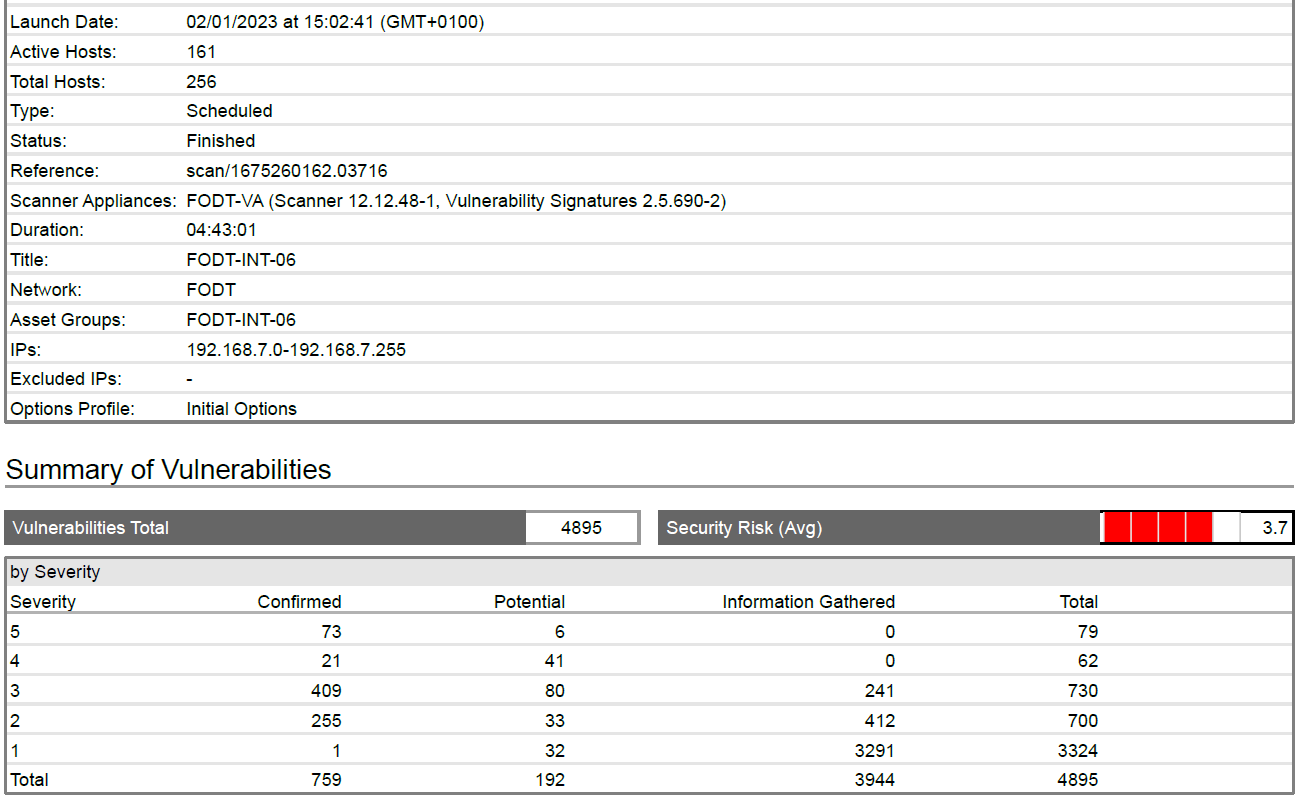
\includegraphics[width=1\linewidth]{images/FODT-INT-06_1.png}
    \caption{}
    \label{fig:fodt-int-06_1}
\end{figure}

\begin{figure}[t]
    \centering
    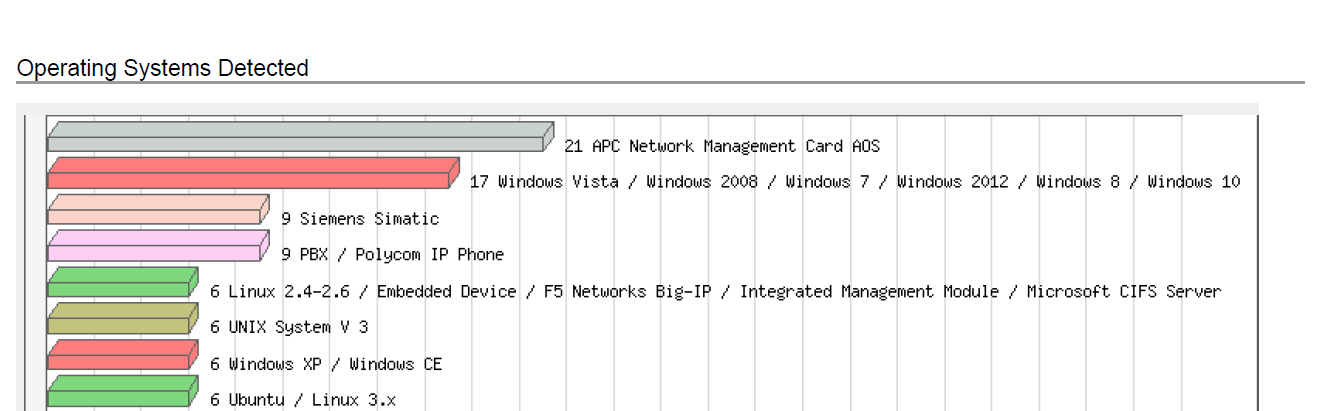
\includegraphics[width=1\linewidth]{images/FODT-INT-06_2.png}
    \caption{}
    \label{fig:fodt-int-06_2}
\end{figure}

\begin{figure}[t]
    \centering
    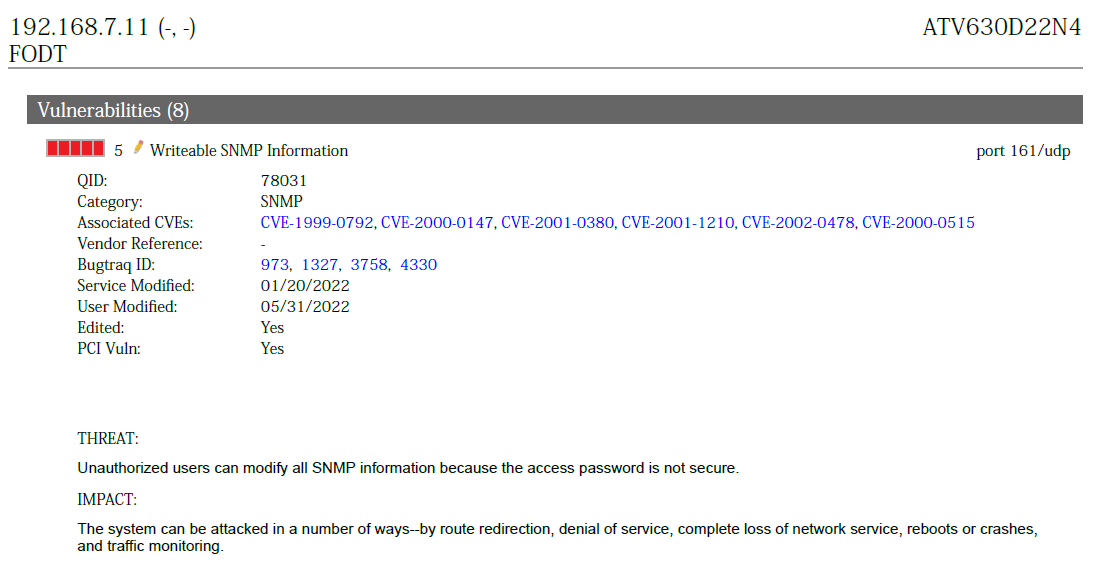
\includegraphics[width=1\linewidth]{images/FODT-INT-06_3.png}
    \caption{}
    \label{fig:fodt-int-06_3}
\end{figure}


L’analisi di questo target sembra aver rilevato molti dispositivi secondari come telefoni IP e schede di gestione (Figura \ref{fig:fodt-int-06_2}), alcuni dispositivi Linux, alcune postazioni Windows, e probabilmente dei macchinari industriali (es. 192.168.7.44).
L’analisi ha rilevato molte vulnerabilità di criticità media e alcune di severità alta.

Le vulnerabilità più occorrenti riguardano il servizio SNMP il quale anche in questo caso risulta abilitato in scrittura (anche in molti dispositivi secondari) e configurato con una \textit{community string} debole (Figura \ref{fig:fodt-int-06_3}).

Sono stati rilevati inoltre vari host (tra i quali presumibilmente server e workstations) con protocolli di sicurezza deboli (TLS v1.0 e v1.1).
\\ Alcune postazioni Windows (192.168.7.176, 192.168.7.222) espongono un servizio di accesso remoto (VNC) configurato in modo da permettere un accesso alla componente server senza autenticazione.

Si segnala inoltre che i dispositivi Windows 192.168.7.30 e 192.168.7.142 presentano gravi vulnerabilità, risultanti dall’uso del sistema operativo Windows 7. Tale sistema operativo infatti non è più supportato ufficialmente da Microsoft, quindi non riceverà più aggiornamenti alla sicurezza. Si proceda urgentemente all’aggiornamento di tali asset.

Il target in questione possiede una scarsa omogeneità in termini di tipologia di asset e dispositivi. Oltre alla disattivazione dei servizi esposti non strettamente necessari, si consiglia fortemente di suddividere questa rete in più sottoreti più omogenee, così da prevenire al meglio la diffusione di un possibile attacco da dispositivi secondari a infrastrutture più importanti.

\subsection{Target FODT-INT-13} \label{fodt-int-13} \textbf{\textit{Figura \ref{fig:fodt-int-13_1}}}


\begin{figure}[t]
    \centering
    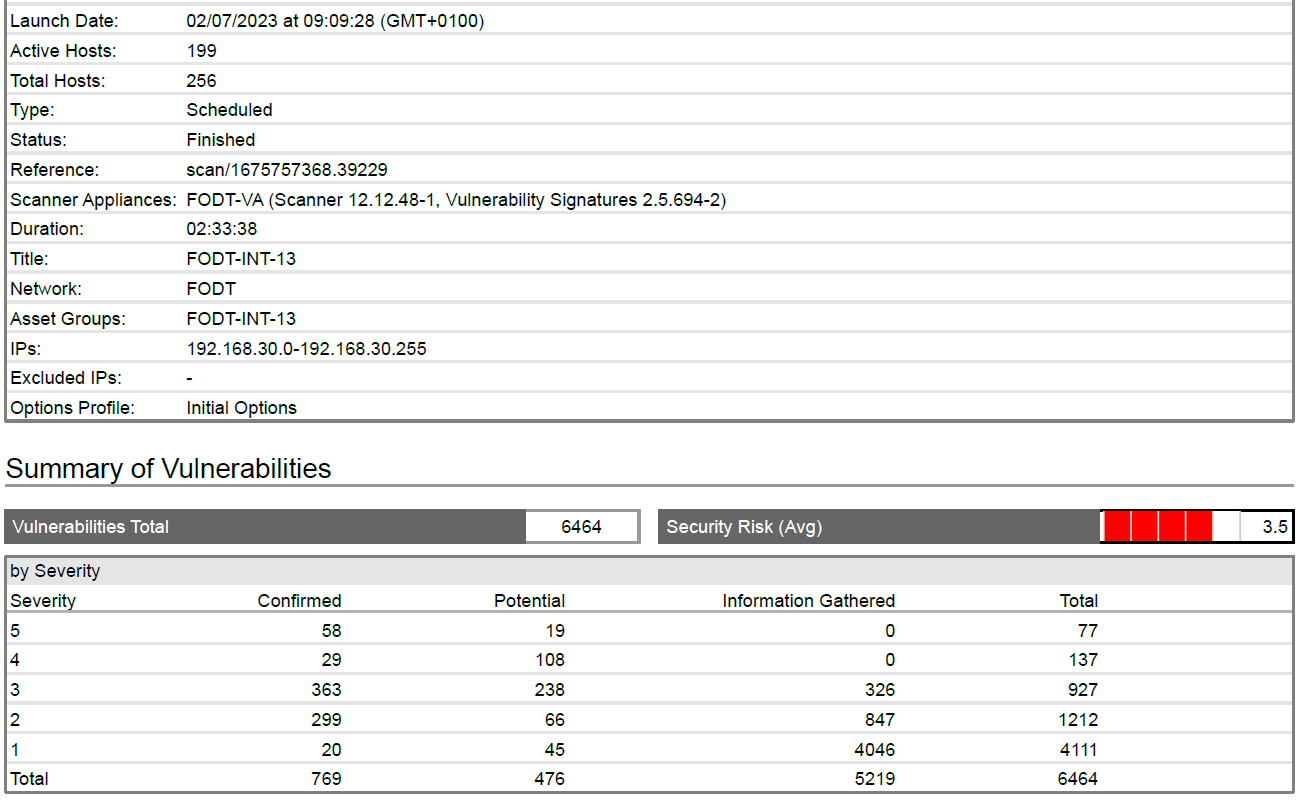
\includegraphics[width=1\linewidth]{images/FODT-INT-13_1.png}
    \caption{}
    \label{fig:fodt-int-13_1}
\end{figure}

\begin{figure}[t]
    \centering
    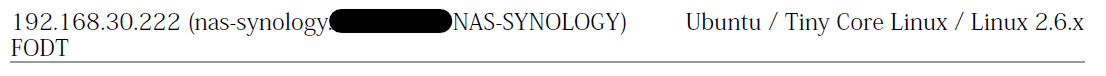
\includegraphics[width=1\linewidth]{images/FODT-INT-13_2.png}
    \caption{}
    \label{fig:fodt-int-13_2}
\end{figure}

\begin{figure}[t]
    \centering
    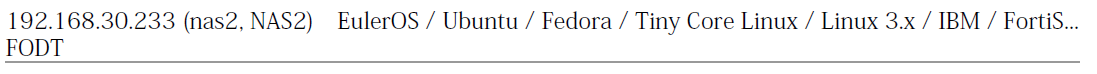
\includegraphics[width=1\linewidth]{images/FODT-INT-13_3.png}
    \caption{}
    \label{fig:fodt-int-13_3}
\end{figure}

L’analisi di questo target ha rilevato una grande quantità di vulnerabilità di livello medio e significative vulnerabilità di severità critica. Il target è costituito in prevalenza da dispositivi Windows.

La principale criticità trovata riguarda l’utilizzo di sistemi operativi deprecati e obsoleti in vari host come Windows XP e Windows 7.
Tra questi vi sono gli host 192.168.30.17, 192.168.30.27, 192.168.30.37 e 192.168.30.240 i quali presentano molte vulnerabilità critiche note nei protocolli di condivisione di dati SMB e di accesso remoto RDP. Tali vulnerabilità sono molto pericolose dato che sono noti vettori di \textit{ransomware}, virus che cifrano l’intero disco fisso del dispositivo, si diffondono autonomamente su altri sistemi vulnerabili e richiedono un riscatto per lo sblocco dei file cifrati.

Alcuni host (192.168.30.65, 192.168.30.85, 192.168.30.129) possiedono delle configurazioni deboli dei servizi di sicurezza e crittografia del traffico di rete (SSL/TLS).

Un altro servizio esposto vulnerabile trovato (es 192.168.30.38 e 192.168.30.46) è il protocollo che permette il trasferimento di file sulla rete (FTP). Si consideri la disattivazione di tale servizio se non necessario.

Sono stati rilevati due dispositivi (192.168.30.222 e 192.168.30.233) che, dai nomi di dominio, sembrano essere NAS (Figure \ref{fig:fodt-int-13_2} e \ref{fig:fodt-int-13_3}).

Il target in questione necessita di \textit{remediation} urgente (in prevalenza aggiornamento dei sistemi). La presenza di sistemi operativi obsoleti e insicuri unita alle deboli configurazioni di sicurezza di molti host sono infatti una vera minaccia all’integrità dell’intera rete.

\subsection{Target FODT-INT-31} \textbf{\textit{Figura \ref{fig:fodt-int-31_1}}}


\begin{figure}[t]
    \centering
    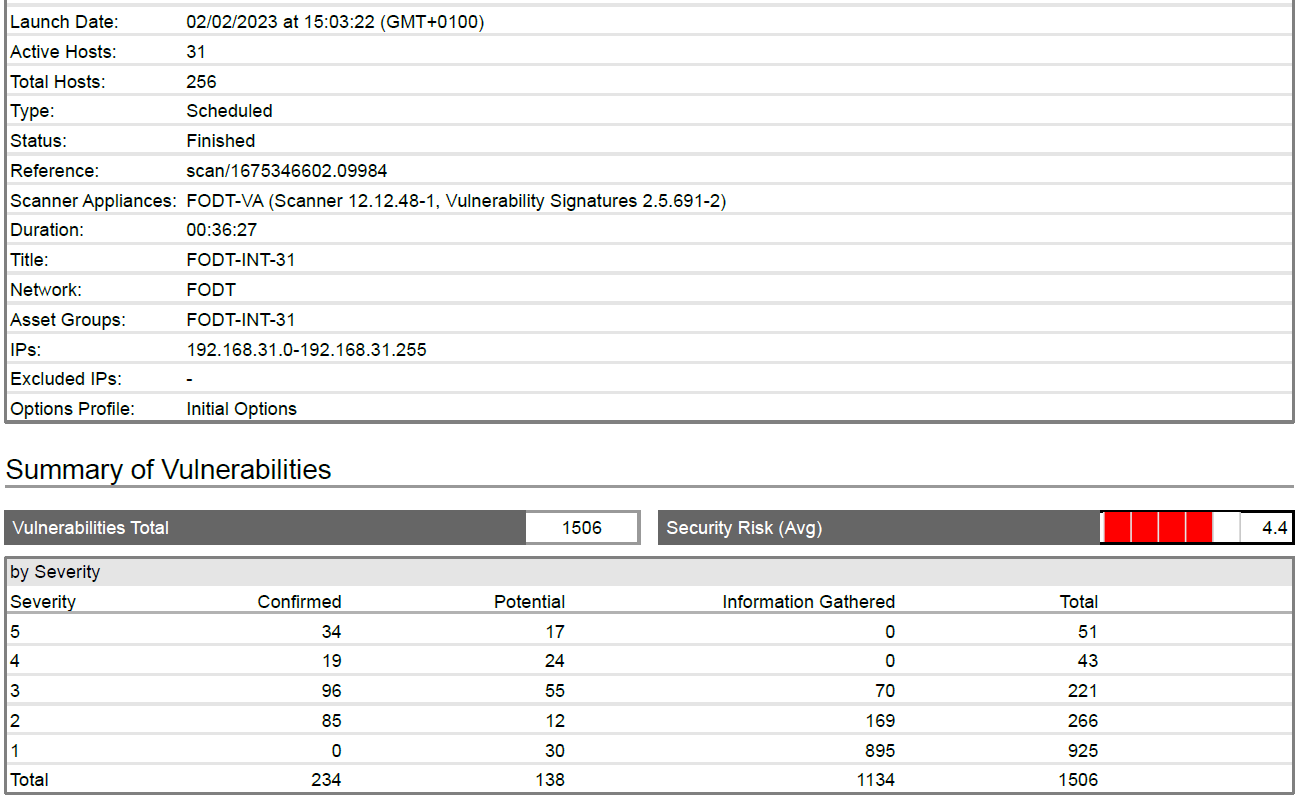
\includegraphics[width=1\linewidth]{images/FODT-INT-31_1.png}
    \caption{}
    \label{fig:fodt-int-31_1}
\end{figure}

\begin{figure}[t]
    \centering
    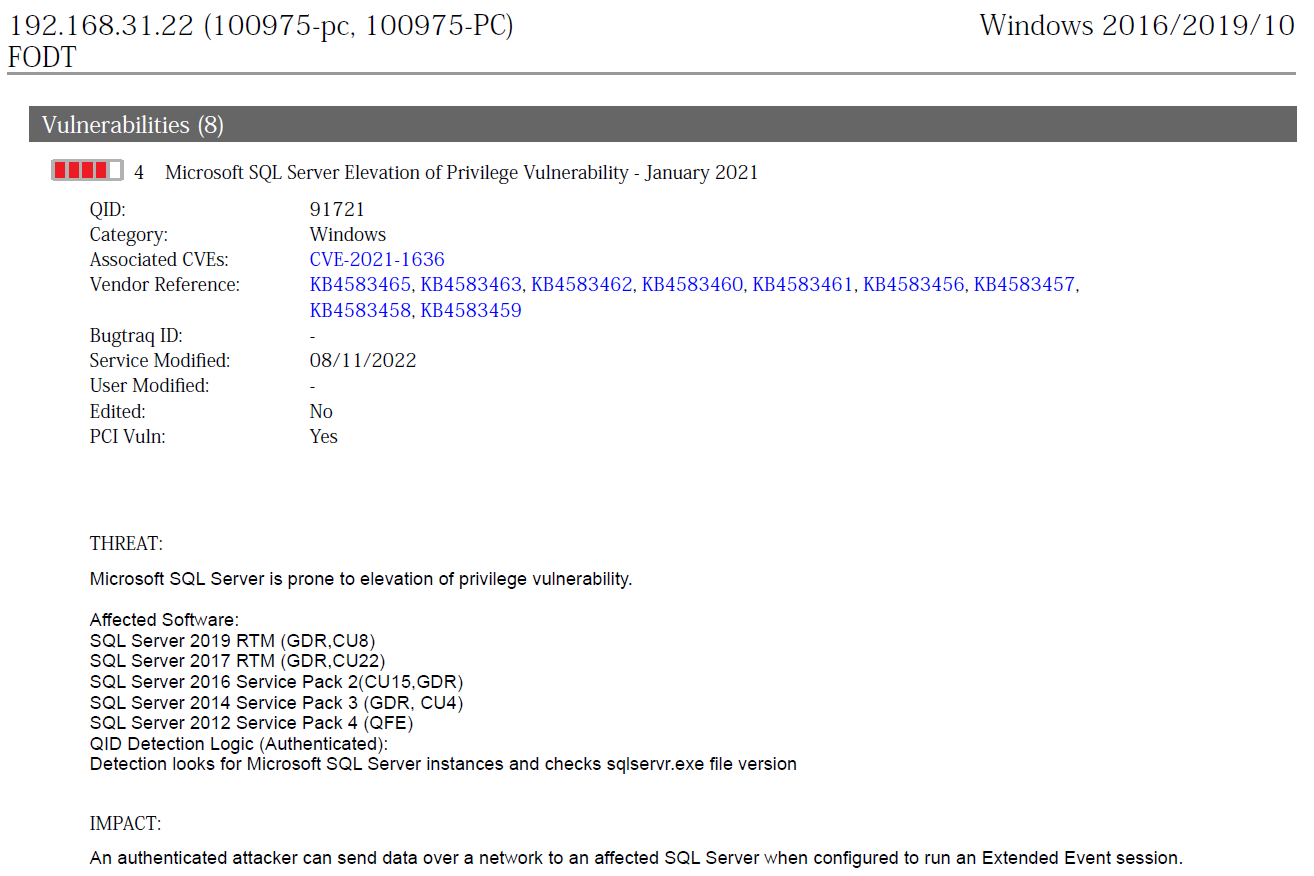
\includegraphics[width=1\linewidth]{images/FODT-INT-31_2.png}
    \caption{}
    \label{fig:fodt-int-31_2}
\end{figure}


L’analisi di questo target ha rilevato un grande quantitativo di vulnerabilità di livello medio e significative vulnerabilità di severità critica. Il target è costituito in prevalenza da dispositivi Windows.

Come per il target FODT-INT-13 la principale criticità trovata riguarda l’utilizzo di sistemi operativi deprecati e obsoleti in vari host come Windows XP e Windows 7.
Gli host 192.168.31.6, 192.168.31.9 e 192.168.31.24, ad esempio, presentano molte vulnerabilità critiche note nei protocolli di condivisione di dati SMB, accesso remoto RDP e di sicurezza SSL/TLS.

Gli host 192.168.31.7, 192.168.31.8, 192.168.31.20 e 192.168.31.22 risultano essere database SQL (Figura \ref{fig:fodt-int-31_2}). Tutti gli asset espongono in rete, precisamente attraverso la porta 1433, un servizio che permette di interfacciarsi con il database, vulnerabile. In particolare la vulnerabilità appartiene alla categoria del \textit{privilege escalation}, ovvero permette ad un utente o ad un'applicazione concepita inizialmente per avere accessi e privilegi limitati di ottenere accesso non autorizzato a risorse.

Anche questo target necessita di \textit{remediation} urgente. È necessario procedere con la messa in sicurezza degli asset che espongono servizi SQL server e l'aggiornamento dei sistemi obsoleti.

\subsection{Considerazioni finali}
Il livello generale di rischio è medio. La maggior parte delle criticità gravi sono presenti nei target FODT-INT-01a, FODT-INT-06, FODT-INT-13 e FODT-INT-31. Queste reti sono un pericolo per l’intera infrastruttura aziendale in quanto costituiti da molti sistemi obsoleti e con gravi e note vulnerabilità. Si raccomanda di predisporre un piano di remediation per correggere in ordine di priorità le criticità più gravi e a seguire quelle intermedie. Molte delle vulnerabilità dovrebbero poter essere corrette tramite aggiornamenti e patching, altre richiederanno correzioni alle configurazioni.

Un’attenzione particolare va posta sull’architettura della rete, volta a verificare (se non già implementata) che almeno le infrastrutture di backup (NAS o simili), ma possibilmente anche quelle di management (es. ESXi), siano mantenute separate dall’infrastruttura di produzione (server e client), per evitare o limitare il rischio di attacco trasversale (ad esempio per un \textit{ransomware}) sui dati di produzione e anche sui backup.

Considerare inoltre, a seguito di una scrupolosa analisi, di disabilitare, soprattutto nei dispositivi secondari, i servizi esposti non strettamente necessari, ad esempio servizi di accesso e gestione remota come VNC, RDP o SNMP, così da limitare il più possibile lo spazio di manovra di un possibile attaccante.


\chapter{Metodi di \textit{remediation}} \label{cap:part-3}

Verranno ora descritte possibili soluzioni alle problematiche riscontrate nelle precedenti analisi e alcune \textit{best practices} al fine di irrobustire la sicurezza dell'infrastruttura di rete aziendale.

\section{Compartimentazione della rete}

Segmentare una rete significa suddividere logicamente il complesso dell'infrastruttura di rete in più reti distinte fra di loro. Invece, di avere un'unica grande rete, ad esempio di classe B\footnote{Gruppo di indirizzamenti IP da 128.0.0.0 a 191.255.0.0 con \textit{subnet mask} fissa a 255.255.0.0, quindi con 16 bit riservati alla rete e 16 per gli host.}, si creano \textit{subnet} più piccole ognuna dedicata ad un proprio ambito, come la rete delle \textit{workstations}, dei server, di \textit{management} o dei backup. In questo caso il termine \textit{subnet} non identifica necessariamente un indirizzamento derivato da una rete con \textit{subnet mask} minore\footnote{Ad esempio la rete 192.168.80.0/20 è sottorete di 192.168.0.0/16.}. La compartimentazione di un'infrastruttura informatica può essere eseguita anche con un approccio "orizzontale", ovvero tramite l'utilizzo di identificatori di rete diversi ma con stessa \textit{subnet mask}, ad esempio 192.168.5.0/24, 192.168.10.0/24 e 192.168.15.0/24.

La segmentazione di rete permette di gestire più opportunamente e organizzare gli asset in specifiche sottoreti in base alla propria affinità con lo scopo che essi ricoprono. Questo permette di implementare logiche di controllo degli accessi tra le sottoreti in modo da rispecchiare le \textit{policy} definite dall'azienda insieme agli eventuali consulenti IT. Ad esempio si potrebbe stabilire che due reparti appartenenti a due reti diverse non possano interagire oppure solo uno dei due può accedere alle risorse dell'altro, è possibile far comunicare specifici host di una rete con uno o più specifici server appartenenti alla propria rete isolata, o ancora è possibile implementare una rete dedicata completamente a macchinari industriali o alla gestione e manutenzione degli apparati di rete, come switch, NAS, server o access point.

Il dispositivo che si occupa di gestire le sottoreti e il relativo traffico è il firewall. Esso permette di creare regole che consentono o meno il traffico in entrata su un'interfaccia e in uscita su un'altra a seconda dell'indirizzo IP di sorgente e destinazione ma anche a seconda del servizio (quindi della porta) che si tenta di contattare. Si può decidere ad esempio che la rete delle postazioni di lavoro possa accedere al \textit{file server} solamente attraverso il servizio SMB, oppure che la rete guest possa esclusivamente uscire in internet attraverso i protocolli HTTP, HTTPS e servizi mail SMTP e SMTPS.
\\ Il firewall, quindi, offre una gestione ottimale e centralizzata delle interfacce di rete e perciò, in una rete aziendale, il dispositivo che dovrebbe fare \textit{routing} è appunto il firewall. Alcuni firewall operano a livello applicativo del modello ISO/OSI e sono quindi in grado di analizzare e filtrare il traffico tra le sottoreti e da Internet (più precisamente è in grado di leggere e analizzare il \textit{payload} di ogni pacchetto che transita tramite esso).

Una corretta segmentazione, quindi, oltre a permettere una gestione più organizzata e intuitiva della rete, consente di isolare l'eventuale attacco limitando il numero di dispositivi compromessi. Ciò che si vuole evitare, infatti, sono i cosiddetti movimenti laterali di un attaccante all'interno della rete, ovvero la possibilità per l'attaccante di muoversi di host in host vulnerabile verso obiettivi sempre più sensibili. Si prenda come esempio una rete nella quale risiedono anche dispositivi \textit{Internet of Things}. Questi asset solitamente necessitano di una configurazione che permetta di essere raggiunti da remoto e quindi di essere esposti fuori dalla rete locale. Spesso questi dispositivi secondari non sono mantenuti a dovere, ed essendo per loro natura vulnerabili (in quanto dispositivi ancora relativamente recenti) vengono presi frequentemente di mira. Se all'interno della loro stessa rete risiedono anche dispositivi di produzione come \textit{workstations} e macchinari industriali allora è logico aspettarsi che prima o poi tali dispositivi possano essere compromessi mediante un attacco originato da asset secondari, siano essi dispositivi IoT, stampanti o telefoni IP.

Come si è potuto notare dall'analisi dei target, la rete presa in esame non presenta una segmentazione ottimale, nonostante il documento della \textit{target definition} (Figura \ref{fig:target_definition_int}) presenti invece una compartimentazione e un numero adeguato di sottoreti.

Al \textit{target} FODT-INT-06 (Paragrafo \ref{fodt-int-06}), che fa riferimento alla sottorete 192.168.7.0/24, appartengono molti dispositivi di natura diversa: \textit{client} Windows (obsoleti), sistemi Linux (che possono comprendere una grande varietà di dispositivi, da telefoni IP a web server) e schede di gestione.

Un'altra sottorete pericolosamente esposta ad attacchi è la 192.168.30.0/24 (\textit{Target} FODT-INT-13, Paragrafo \ref{fodt-int-13}). In questa rete risiedono infatti sia sistemi operativi obsoleti come Windows XP e Windows 7, che dispositivi NAS di archiviazione. Potenzialmente, quindi, basterebbe che un utente distratto o poco consapevole aprisse un allegato di una mail di \textit{phishing} per compromettere anche i sistemi di backup (Nel caso in cui tali dispositivi fossero dedicati a queste operazioni).

Le sottoreti vengono configurate sul firewall sotto forma di interfacce virtuali, chiamate VLAN \cite{cybercreativa}\cite{reti}. Oltre all'identificatore di rete (ad esempio 172.16.20.0/24) viene associato anche il cosiddetto VLAN ID, ovvero un numero da 1 a 4096. Questo identificativo, che viene aggiunto al \textit{frame} Ethernet, permette alle rispettive sottoreti di essere propagate anche sugli switch. Essi, essendo dispositivi appartenenti al livello 2 nello stack ISO/OSI, non permettono il routing dei pacchetti e pertanto utilizzano tale ID per decidere quali client possono parlarsi fra di loro. Di base qualsiasi host appartenente ad una specifica VLAN è autorizzato a comunicare con tutti gli host che risiedono nella VLAN con stesso ID.

L'associazione fra dispositivo e VLAN avviene fisicamente attraverso il collegamento con una porta dello switch. Ogni porta può essere configurata per far passare una specifica VLAN (ovvero \textit{frame} con quello specifico ID) oppure qualsiasi VLAN (queste porte sono definite di \textit{trunk} e solitamente vengono attivate per il collegamento con un altro switch o un qualsiasi dispositivo che permetta l'inoltro dei \textit{frame}).

È buona norma inoltre tenere disabilitate le porte libere inutilizzate. Così facendo si evitano inconvenienti come \textit{loop} di rete a seguito del collegamento improprio di un dispositivo di rete ma anche accessi non autorizzati all'interfaccia di gestione dello switch. 

Nel caso dei \textit{target} in questione vi è pertanto la necessità di rivalutare il modo nel quale le componenti della rete si interfacciano fra di loro andando a riconfigurare le interfacce degli switch e le eventuali regole di firewall. Priorità assoluta va data all'infrastruttura di backup.

\section{Isolamento dei backup}
I backup costituiscono una componente fondamentale non solo dell'infrastruttura informatica ma dell'intera azienda. Essi, se configurati e mantenuti a dovere, garantiscono la possibilità di ripristinare le configurazioni e i dati dei sistemi che compongono l'infrastruttura in caso di cancellazioni volontarie o involontarie da parte degli utenti, compromissione e cifratura dei dati a seguito di attacchi informatici oppure nella malaugurata evenienza di incidenti come infiltrazioni d'acqua e incendi.

Data la sua importanza, l'infrastruttura dei backup viene spesso presa di mira come primo obiettivo negli attacchi informatici\footnote{Dai risultati del report "\textit{2023 GLOBAL REPORT: 
RANSOMWARE TRENDS}" \cite{veeam}, eseguito da Veeam considerando 1200 vittime e 3000 \textit{cyber} attacchi, è emerso che nel 2022 il 93\% degli attacchi mirava principalmente ai \textit{repository} di backup.}, di conseguenza è necessario prevedere un accurato isolamento di tali sistemi e meccanismi di riserva per il salvataggio delle copie di sicurezza.

Prenderemo in considerazione lo scenario più comune e ragionevole, ovvero l'esecuzione dei backup su NAS o server dedicati appartenenti, come visto nel paragrafo precedente, ad una VLAN apposita facente riferimento a una specifica classe di indirizzamento.

Definiamo ora i dati che si vogliono proteggere.
\\ Alla base dell'infrastruttura informatica di un'azienda vi è il server fisico\footnote{Per semplicità ne consideriamo uno anche se nella realtà ce ne possono essere multipli, spesso sincronizzati fra di loro a creare un \textit{cluster}.}, un computer ad elevate prestazioni. Tale apparato è dotato di un software di virtualizzazione che permette l'esecuzione e la creazione su di esso di istanze virtuali di sistemi operativi come Windows o Linux. Queste macchine virtuali (VM) rappresentano i server logici ai quali gli utenti finali richiedono servizi e applicativi e tramite i quali viene gestita l'infrastruttura di rete.

I sistemi di backup dovrebbero provvedere a mettere in sicurezza le singole macchine virtuali eseguendone periodiche copie. Solitamente questa operazione viene eseguita da una macchina virtuale dedicata esclusivamente all'esecuzione dei backup, quindi con un sistema operativo ad hoc, oppure da una \textit{virtual machine} Windows o Linux avente il software di backup. Queste saranno le uniche VM autorizzate, tramite regole di firewall, ad interfacciarsi con i \textit{repository} di backup e, in quanto tali, avranno la necessità di essere costantemente monitorate ed aggiornate alle ultime \textit{patch} di sicurezza. Lo scenario migliore consiste nel vietare qualsiasi connessione a internet sia in entrata che in uscita. Perciò, per rendere possibile l'accesso agli amministratori, invece di attivare un \textit{agent} sulla macchina per renderla visibile da remoto, si abilitano sul firewall esclusivamente le connessioni da uno specifico server della rete di \textit{management} verso la sola porta HTTPS del server di gestione dei backup. Il supporto sul quale vengono effettuati i backup, invece, può e deve essere completamente isolato dall'esterno verificando accuratamente che non vi siano servizi attivi esposti in rete e che la sottorete di backup nel quale risiede il \textit{repository} non abbia accesso a internet.

Riassumendo, la macchina virtuale di backup, appartenente alla rete fidata di \textit{backup}, richiede all'host di virtualizzazione l'accesso in lettura delle VM installate su di esso, tramite l'apertura di determinate porte sul firewall, e scrive i dati nel server di backup accedendo con un utente dedicato. (Figura \ref{fig:backup})

\begin{figure}[t]
    \centering
    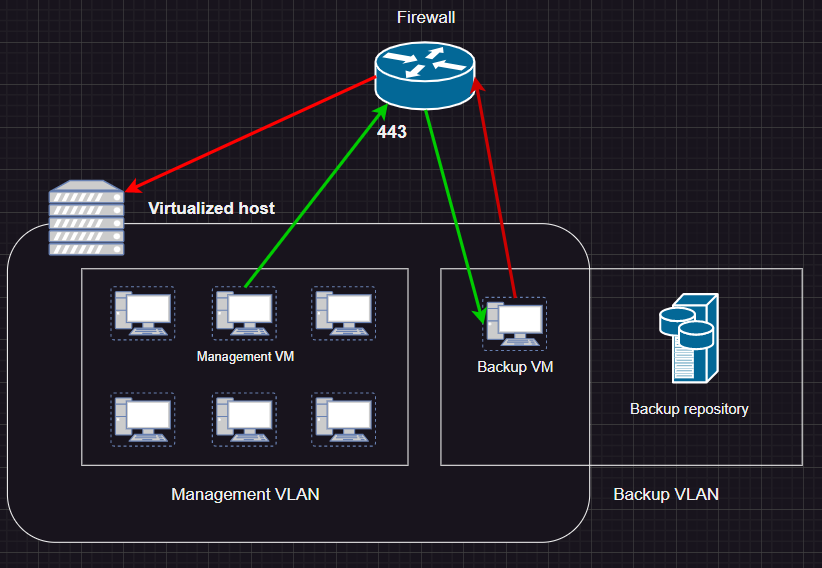
\includegraphics[width=1\linewidth]{images/backup.png}
    \caption{: infrastruttura di backup}
    \label{fig:backup}
\end{figure}

Il punto debole di questo sistema di backup risiede nel fatto che la VM che esegue l'operazione, pur essendo l'unica in grado di contattare il supporto di backup, se violata rischia di invalidare l'integrità del \textit{repository}. Una strategia più sicura, ma anche più costosa in termini economici e di performance, consiste nell'affidarsi a un servizio terzo e delegare l'esecuzione del backup ad un agente installato direttamente sui server e che invia i dati al supporto di backup nei datacenter proprietari del produttore del servizio. Così facendo si è in grado di delegare la gestione delle copie e la relativa sicurezza. Il backup inoltre verrebbe portato \textit{off-site} e un eventuale \textit{hacker} all'interno della rete aziendale non avrebbe quindi accesso ad alcun \textit{repository}.

Anche quest'ultimo approccio, tuttavia, non è ottimale in quanto se si volesse effettuare, ad esempio, un ripristino veloce e urgente di una macchina virtuale da 5 Terabyte, ciò non sarebbe pratico per via della grande larghezza di banda che questa operazione richiederebbe.

Lo scenario migliore, perciò, è avere più sistemi di backup complementari, ovvero unire le strategie precedentemente esposte. È possibile limitare il rischio di perdita dei dati, ad esempio, implementando meccanismi di backup di secondo o terzo livello, ed effettuando periodicamente una copia del backup primario su un supporto diverso, programmando quest'ultimo per attivarsi solamente in questi momenti e rimanere spento il resto del tempo. I due (o più) supporti di backup potrebbero, inoltre, appartenere a due sottoreti diverse, in modo tale da dissuadere un eventuale attaccante nel cercare ulteriori sistemi di \textit{storage} e indurlo invece a ritenere che non siano presenti altri \textit{repository} di backup.
\\ A questo sarebbe opportuno aggiungere un backup \textit{off-site}, ad esempio in cloud.

Secondo l'Articolo 32 del GDPR, inoltre, l'azienda dovrebbe predisporre periodiche verifiche riguardo il funzionamento e l'integrità dei sistemi di backup implementati, testando, insieme al loro corretto isolamento, anche le procedure di ripristino delle copie di sicurezza \cite{backup}.

\section{Disattivazione e messa in sicurezza dei servizi esposti}

Come spiegato in precedenza, ogni servizio o programma in ascolto su un sistema informatico rappresenta potenzialmente una porta aperta nella propria rete, sia tecnicamente che figurativamente.

La prima accortezza da avere è verificare che sul firewall non vi siano regole che permettano di instaurare connessioni dall'esterno del perimetro aziendale al suo interno, tramite qualsiasi servizio. Nel caso in cui ci fosse invece reale bisogno di concedere l'accesso a un sistema interno della rete, ad esempio un cliente che ha necessità di accedere ad un server FTP interno, sarà opportuno configurare la regola in modo da consentire le connessioni esclusivamente a determinati IP pubblici che andranno periodicamente verificati e, se non più validi (nel caso in cui ad esempio il sistema remoto cambiasse il proprio indirizzo pubblico) esclusi.

Se invece si volesse consapevolmente offrire dei servizi su internet, ad esempio attraverso dei mail server proprietari, la scelta migliore e più sicura consiste nel collocare i sistemi che espongono tali servizi in una DMZ, ovvero DeMilitarized Zone. Questa è a tutti gli effetti un'interfaccia di rete aggiuntiva offerta dal firewall e permette di separare completamente il traffico di rete dei sistemi esposti in internet da quello della rete LAN privata interna all'azienda. Sul firewall verrà quindi configurata una regola che inoltra le connessioni provenienti da internet verso l'interfaccia in questione tramite le porte corrispondenti ai servizi che si vogliono esporre.

Per permettere la fruizione dei servizi erogati dalla intranet aziendale come l'accesso alle cartelle di rete condivise o ai server interni anche da parte di dipendenti, fornitori o clienti che risiedono su reti remote, è necessaria una VPN, in particolare è necessaria la configurazione di una SSL VPN. Tale tipologia di VPN si basa sull'autenticazione da parte degli utenti su un client installato sulla propria postazione e configurato in modo da dirottare e inoltrare il traffico in uscita verso un gateway specifico che solitamente coincide con il firewall dell'azienda. Così facendo i pacchetti di rete vengono crittografati a partire dal livello di trasporto e alla postazione connessa viene assegnato un indirizzo IP appartenente alla sottorete degli utenti SSL VPN. Sarà poi cura degli amministratori di rete concedere ai singoli utenti o a quest'ultima \textit{subnet} l'accesso ai vari servizi interni. 

L'esempio migliore e più esplicativo riguarda l'utilizzo del servizio \textit{Remote Desktop Protocol} (RDP) per il collegamento remoto a un determinato computer tramite interfaccia grafica. In ambienti lavorativi è un applicativo molto usato in quanto permettere ai dipendenti di poter lavorare sulle proprie postazioni in ufficio pur essendo fuori sede. Comunemente viene adibito un server apposito, definito solitamente \textit{terminal server}, per ricevere le connessioni dagli utenti remoti i quali si autenticano con le proprie credenziali del dominio aziendale. Data la notevole funzionalità che RDP offre e la sua nota vulnerabilità ad attacchi informatici gravi\footnote{\textit{BlueKeep} (CVE-2019-0708) è una vulnerabilità di RDP che permette l'esecuzione di codice da remoto}, configurare sul firewall un \textit{port forwarding} che inoltri le chiamate da internet all'IP pubblico aziendale attraverso la porta RDP (3389) verso il terminal server, non è assolutamente una pratica ideale. Ciò che normalmente si implementa è una autenticazione aggiuntiva alla rete interna aziendale tramite la VPN. In questo modo sarà necessario per il terminal server esporre la porta RDP solamente nella sottorete degli utenti autenticati nella VPN.

Può capitare che si voglia mettere in comunicazione due host appartenenti a due reti private remote. Due aziende potrebbero voler collaborare su degli stessi clienti condividendo le stesse risorse e quindi sincronizzare da entrambi i lati le modifiche effettuate sui rispettivi file server. Un modo col quale i due server possono comunicare e trasferire i dati fra di loro è tramite un tunnel SSH. Si attiva su entrambi i server il servizio SSH e lo si configura in modo da permettere l'autenticazione a chiave pubblica vista in precedenza (Paragrafo \ref{fodt-int-01}). Pur essendo SSH un protocollo in sé sicuro grazie all'implementazione della cifratura dei dati trasmessi, è pur sempre un servizio che offre la \textit{shell} di un sistema remoto e un potenziale errore nela sua configurazione come semplicemente l'uso di algoritmi crittografici deboli unito alla sua esposizione in rete non contribuirebbe a rendere la rete aziendale sicura. Inoltre ci sarebbe anche la necessità di fare \textit{port forwarding} sul firewall dalla porta SSH verso il server appartenente alla rete interna, aggiungendo altre possibilità di commettere errori.
\\ La pratica corretta, invece, consiste nel configurare un tunnel VPN \textit{site-to-site} fra le due reti remote sul quale si appoggerà a sua volta il tunnel SSH. Questa tipologia di VPN premette di creare una rotta statica implicita fra le due reti, in modo tale da poter comunicare fra asset diversi in reti distanti fisicamente come se la rete remota si trovasse su un segmento diverso della stessa intranet locale, senza quindi l'ausilio di software VPN \textit{client}. Per avere un ulteriore livello di sicurezza e limitare la superficie di attacco, se come in questo caso vi è la necessità di far comunicare due singoli host, la VPN verrà configurata in modo da permettere la trasmissione dati esclusivamente tra i loro indirizzi IP e non all'intera \textit{subnet} nella quale risiedono.

Proteggere il confine con l'esterno vuol dire difendere gli asset e l'intera rete aziendale da attacchi instaurati da internet, riducendo il valore del vettore di attacco (Paragrafo \ref{metriche}). Di conseguenza si costringe l'attaccante ad agire adescando gli utenti interni alla rete tramite tecniche di \textit{social engineering} ad esempio attraverso mail di \textit{phishing} o attacchi \textit{Man in the Middle}.

Nei target analizzati non sono stati rilevati servizi in ascolto su interfacce pubbliche, tuttavia nella rete interna risultano attivi diversi applicativi.
\\Le aziende dovrebbero seguire una filosofia \textit{zero trust}, ovvero considerare non attendibile e non fidata qualsiasi entità, utente, dispositivo o servizio, anche se in diretta gestione dell'azienda, come la propria rete interna privata \cite{zerotrust}. Bisogna quindi implementare meccanismi che permettano, ogni volta in cui - ad esempio - un utente richiede una certa risorsa, sia all'interno che all'esterno della rete aziendale, di poter:

\begin{itemize}
    \item Verificare la sua identità (anche attraverso metodi di autenticazione multi-fattore), quindi il suo ruolo, il contesto nel quale risiede, ad esempio se apre la connessione da casa o dall'ufficio, e a quale risorsa si sta tentando di accedere;
    \item Controllare e ispezionare i movimenti dell'utente all'interno della connessione attraverso l'analisi dei \textit{log} del traffico di rete o la configurazione di filtri DNS\footnote{Meccanismi di difesa che analizzano il traffico in uscita e bloccano eventuali richieste di connessioni verso specifici domini. In particolare viene bloccata la richiesta DNS da parte del client.} sul firewall. Il sistema potrebbe ad esempio rilevare il tentativo di connessione da parte dell'utente a un sito sconosciuto e registrarne l'evento;
    \item Determinare le politiche di accesso o blocco in base allo scenario formatosi, il ruolo dell'utente, il contesto nel quale sta operando e il rischio che la connessione alla specifica risorsa comporterebbe per l'azienda.
\end{itemize}

Riassumendo, la \textit{policy zero trust} implica che a qualsiasi entità vengano forniti i minimi privilegi necessari per portare a termine il proprio lavoro. Questo si traduce nella pratica con l'implementazione di sistemi per il controllo degli accessi alle risorse, come cartelle condivise o dispositivi di rete, attraverso ad esempio la definizione di \textit{group policy} di dominio\footnote{Regole applicate centralmente a livello di computer o utenti del dominio di rete aziendale. Permettono una grande granularità di configurazione delle postazioni e degli utenti.} e regole di firewall restrittive fra \textit{subnet} e dispositivi diversi (si noti l'importanza di avere una rete segmentata). Mano a mano che l'utente ha un reale e confermato bisogno di accedere a un certo servizio gli si concedono gli opportuni privilegi. Questo sistema influisce certamente con l'operatività e la comodità d'uso dei sistemi produttivi aziendali, in quanto gli utenti non saranno completamente autonomi ma avranno bisogno dell'approvazione del responsabile e il supporto del \textit{team} tecnico per la concessione dei privilegi necessari. Questo, tuttavia, è il prezzo da pagare per avere un'infrastruttura solida, relativamente semplice da gestire e quindi orientata alla sicurezza.
\\ Un possibile scenario di applicazione della metodologia \textit{zero trust} è quello di un utente che tramite il proprio \textit{notebook}, solitamente collegato alla rete cablata, vuole accedere a un servizio, che risiede sul server, attraverso la rete \textit{wireless}. Se queste due tipologie di rete rappresentano due classi di indirizzamento diverse, l'utente inizialmente non dovrebbe poter connettersi utilizzando la rete senza fili, poiché ad esempio non vi è nessuna regola sul firewall che autorizzi le connessioni di transitare attraverso la porta corrispondente al servizio richiesto. Per rispettare quindi il criterio \textit{zero trust}, se l'utente non avesse un reale bisogno di richiedere la risorsa in quello specifico contesto, ma la richiesta fosse solo basata su una presunta comodità, allora la politica aziendale dovrebbe essere quella di non permettere una tale connessione.

Questo approccio è valido anche per i dispositivi, come server o NAS, che non fanno riferimento ad alcuna persona fisica. Se un servizio non è necessario che sia esposto in rete il rimedio più semplice è disattivarlo completamente sul dispositivo, il quale dovrebbe fornire solo gli applicativi di cui si ha realmente bisogno ed offrirli esclusivamente ad un gruppo di utenti limitato. Un'accortezza che si potrebbe avere ad esempio è fare in modo che il NAS di backup non risponda in HTTP nella rete di produzione cosi che non possa essere preso di mira da attacchi \textit{brute force}.

Esempi di servizi rilevati nel \textit{vulnerability assessment} da disabilitare o mettere in sicurezza sono SNMP, il quale in molti target risulta abilitato oltre che in lettura anche in scrittura, i servizi FTP, SMB e RDP. La messa in sicurezza e l'isolamento di questi applicativi consiste nella configurazione di metodi di autenticazione robusti (mediante l'uso di algoritmi crittografici e di \textit{hashing} avanzati e l'uso di password complesse) e, come indicato in precedenza, con l'implementazione di specifiche regole che permettano l'accesso alle risorse solamente ad utenti specifici.


\chapter{Conclusione}

La sicurezza della rete aziendale si deve muovere di pari passo con lo sviluppo e l'evoluzione dell'azienda stessa. Il successo di un'organizzazione è basato su ciò che produce e costruisce nel tempo, ovvero le sue proprietà intellettuali. È quindi interesse dell'azienda sviluppare sistemi e metodologie per prevenire compromissioni alla confidenzialità, integrità e disponibilità dell'infrastruttura aziendale, intesa come insieme di apparati e sistemi di produzione, che consentono di rendere efficienti i processi aziendali, permettono di comunicare con la \textit{extranet}\footnote{L'insieme delle infrastrutture di rete di proprietà dell'azienda (server, NAS, switch e firewall) esterne al perimetro aziendale.} e di offrire servizi anche agli utenti esterni come clienti e partner. Questo dovrebbe costituire un processo continuativo e la sicurezza un investimento invece che un peso.

Considerando la sua estensione e complessità sia in termini di hardware che di software, una rete aziendale non gestita opportunamente espone un'ampia superficie di attacco tramite la quale si verificano i \textit{data breach} e le intrusioni di rete. Ogni postazione di lavoro, a prescindere dall'accortezza dell'utente di cui ne fa uso, ogni \textit{endpoint} di rete o macchinario di produzione, ogni applicativo esposto sia esternamente che internamente, è da considerarsi non affidabile. Per far fronte alla costante espansione delle reti aziendali nel tempo e di conseguenza alla loro superficie di attacco è necessario mettere in atto strategie che permettano di difendere su più livelli l'infrastruttura di rete aziendale. Idealmente un'organizzazione vorrebbe proteggere la propria infrastruttura senza pregiudicare la facilità d'uso dei sistemi produttivi. Tuttavia una rete sicura e robusta ha bisogno di adottare metodi diversi di difesa che vadano a coprire più componenti della rete e che inevitabilmente vanno a impattare sulla praticità e sull'autonomia degli utenti. Regole di firewall, segmentazione di rete, politiche di accesso alle risorse sui server e approcci \textit{zero trust} consentono di avere più strati di difesa sovrapposti in modo da avere sempre un meccanismo di riserva.

Al tempo stesso vi è la necessità di ridurre, monitorare e confinare il più possibile l'insieme delle componenti della rete, sia software che hardware, che possono rappresentare vettori di attacco utilizzati per compromettere l'infrastruttura, ovvero la superficie di attacco della rete aziendale. Il \textit{Vulnerability Assessment} consente di giungere proprio a questa necessità ed è uno strumento che in mano all'azienda permette di creare un inventario degli asset collegati in rete e avere un'idea delle principali debolezze più critiche, andando a scandagliare l'intera rete sia da un punto di vista fisicamente interno ed esterno. Il continuo processo di scansione e analisi dei risultati permette di ripensare i propri processi aziendali sviluppando un'architettura più semplice e organizzata, con chiare e intuitive interazioni fra le componenti. Una minore complessità dell'infrastruttura di rete, infatti, ha il vantaggio di essere più facile da amministrare e gestire, e quindi meno incline ad errori di configurazione.


%% Fine dei capitoli normali, inizio dei capitoli-appendice (opzionali)
\appendix

%\part{Appendici}

\chapter{Interfacce di Qualys}
\label{appendix:a}

\begin{figure}[h]
\centering
    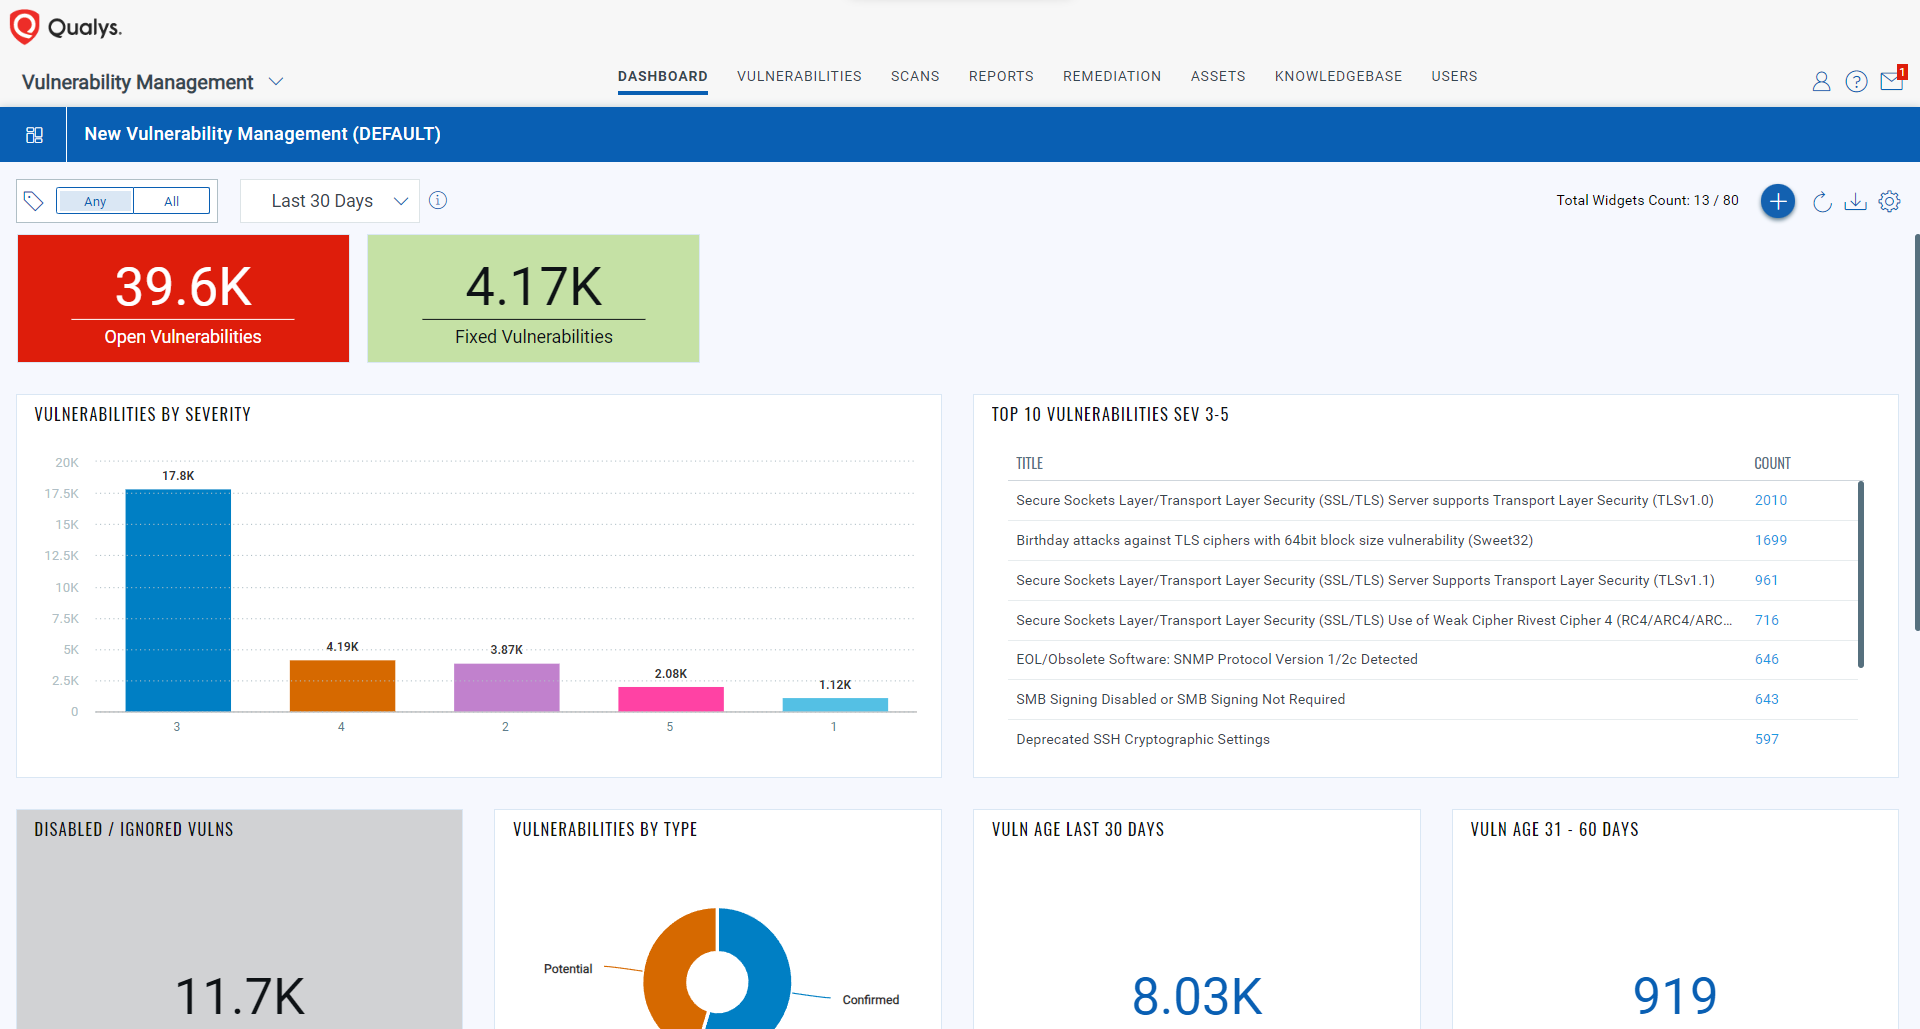
\includegraphics[scale=0.329]{images/qualys_dashboard.png}
    \caption{: \textit{Dashboard}. Visualizza una panoramica, personalizzabile attraverso \textit{widget}, dei risultati e dell'andamento delle scansioni eseguite.}
\end{figure}

\begin{figure}
\centering
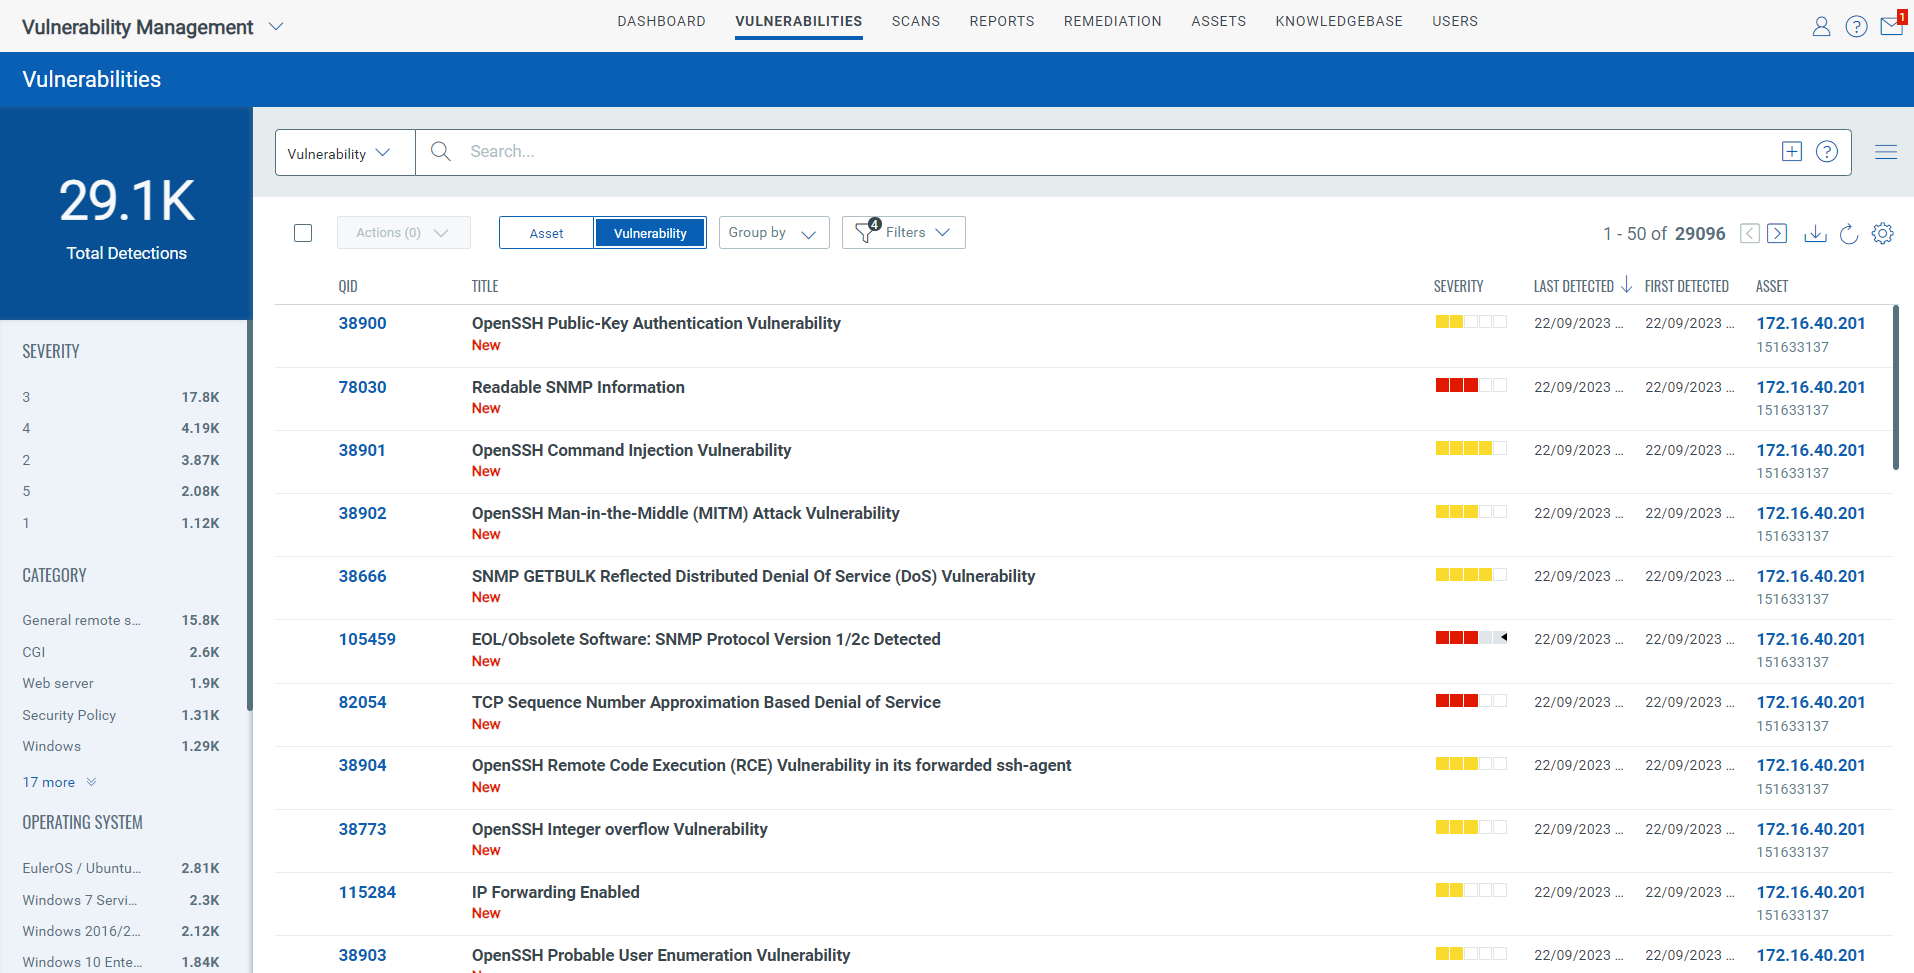
\includegraphics[scale=0.329]{images/qualys_vuln.png}
    \caption{: \textit{Vulnerabilities}. Visualizza una lista delle vulnerabilità trovate nelle ultime scansioni effettuate.}
\end{figure}

\begin{figure}
\centering
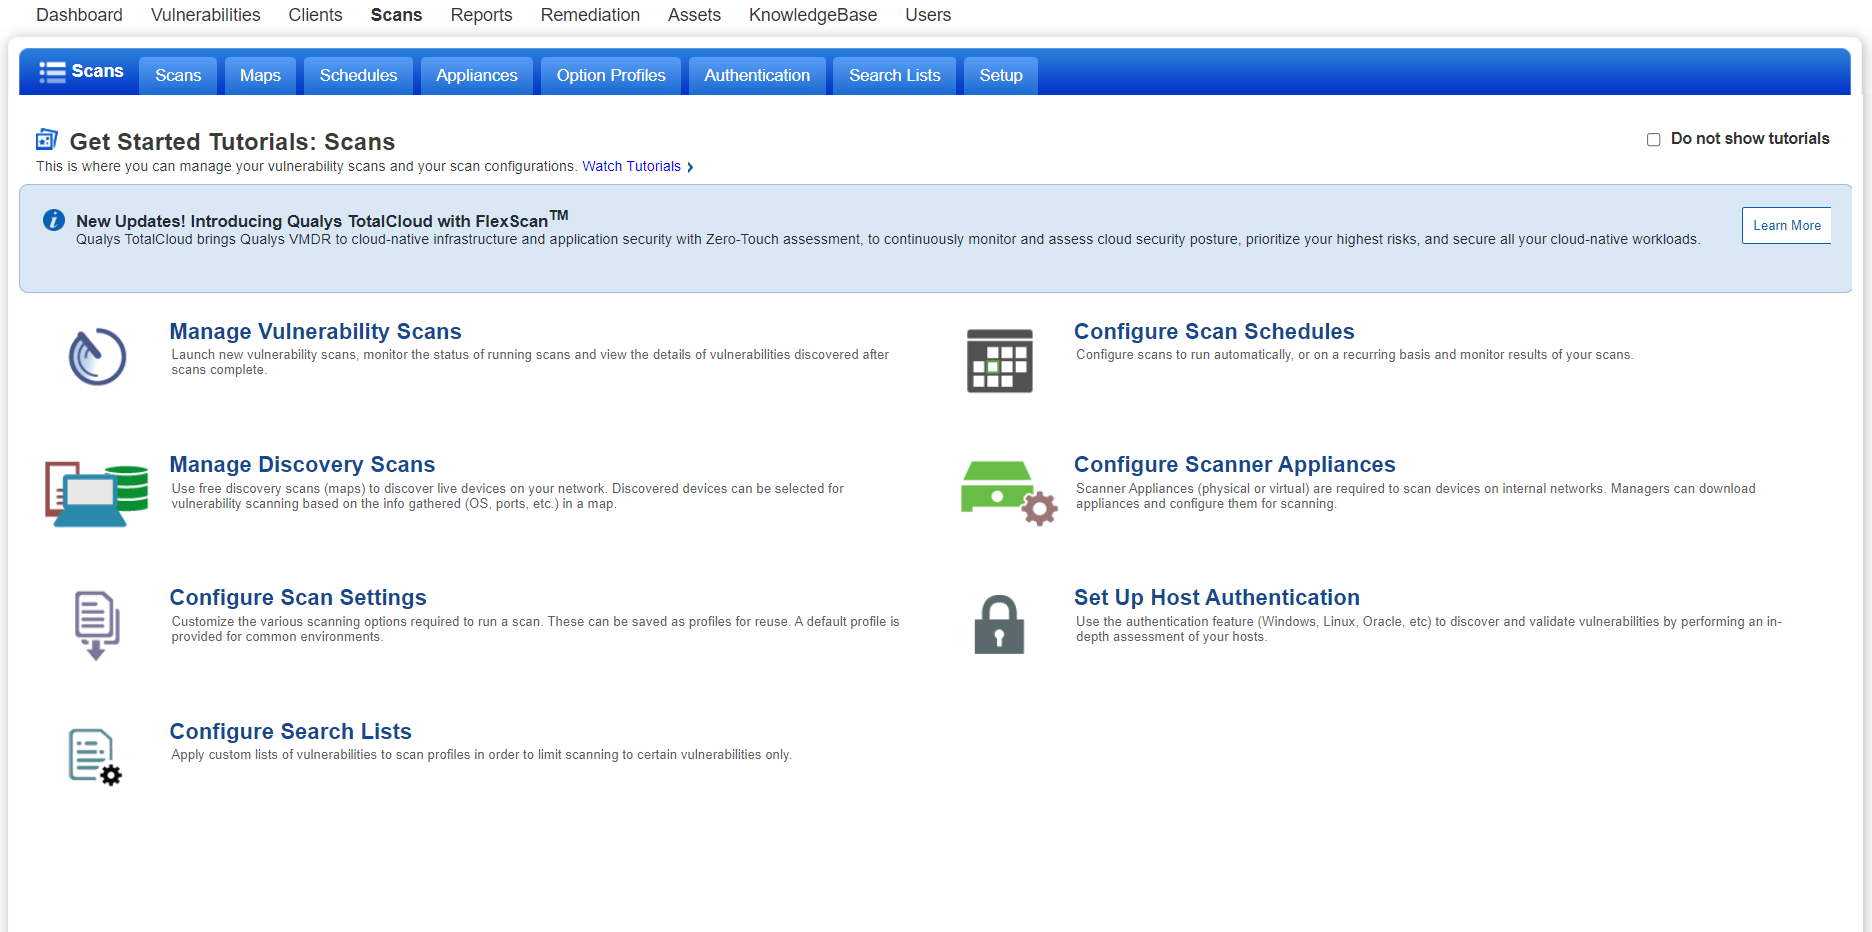
\includegraphics[scale=0.329]{images/qualys_scans.png}
    \caption{: \textit{Scans}. Da qui è possibile configurare, schedulare e monitorare l'esecuzione delle scansioni vere e proprie.}
\end{figure}

\begin{figure}
\centering
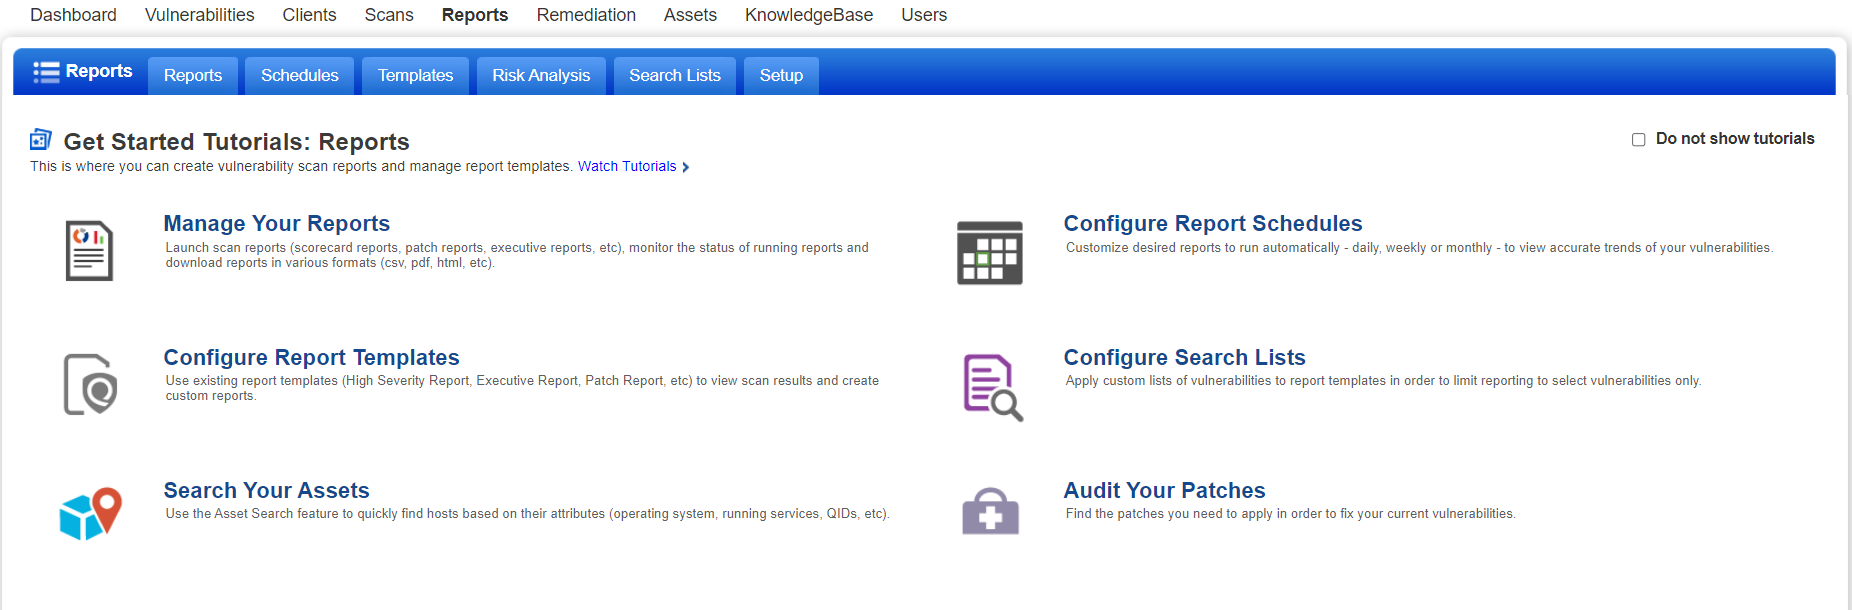
\includegraphics[scale=0.329]{images/qualys_reports.png}
    \caption{: \textit{Reports}. Questa sezione permette di visualizzare i report generati dalle scansioni oppure generarli manualmente. È possibile anche personalizzare i \textit{template} con i quali vengono generati i report.}
\end{figure}

\begin{figure}[!]
\centering
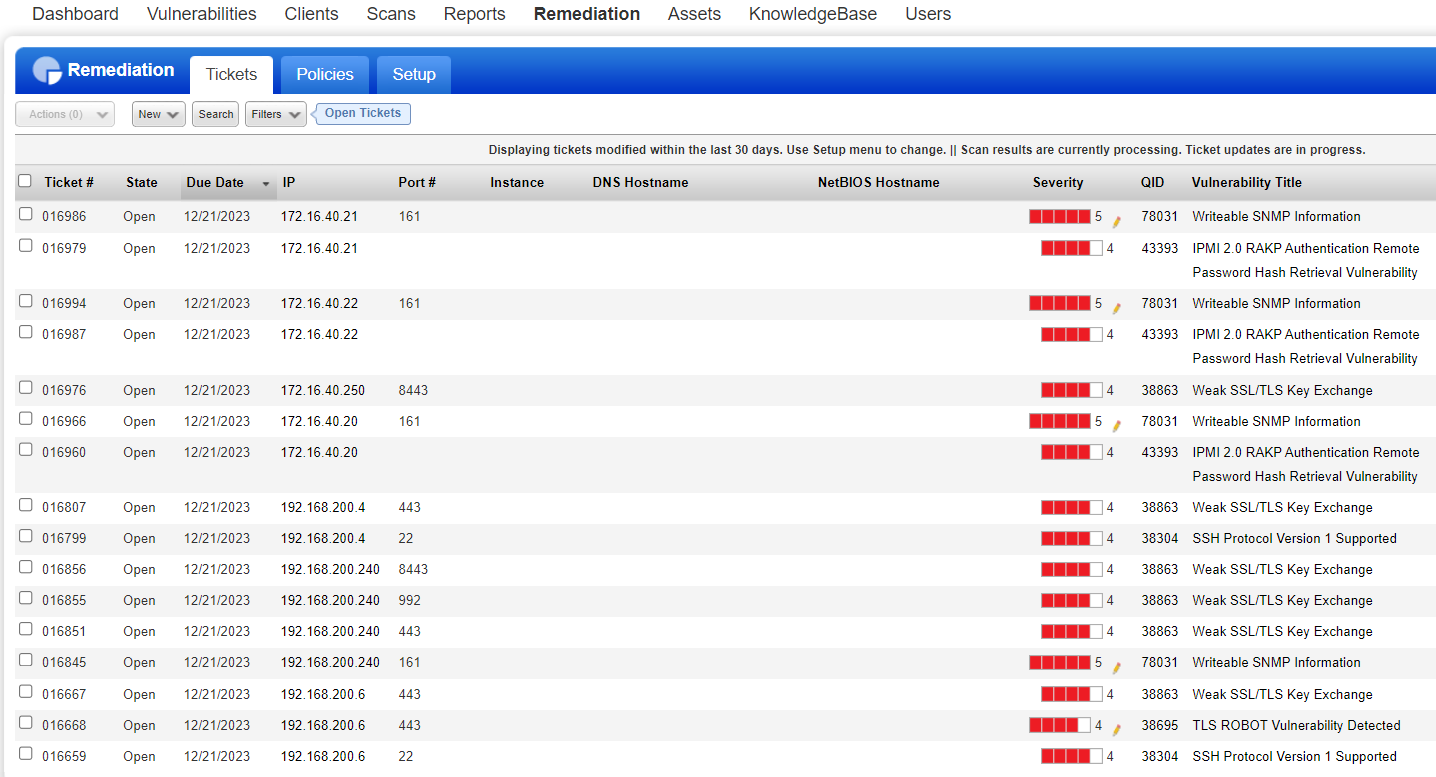
\includegraphics[scale=0.425]{images/qualys_remediation.png}
    \caption{: \textit{Remediation}. Visualizza la lista, con le relative scadenze di risoluzione, delle vulnerabilità trovate nelle scansioni e non ancora risolte.}
\end{figure}

\begin{figure}[h]
\centering
\includegraphics[scale=0.329]{images/qualys_assets.png}
    \caption{: \textit{Assets}. Permette di creare e gestire gli asset e i relativi gruppi che saranno oggetto delle scansioni.}
\end{figure}

\begin{figure}[!]
    \centering
    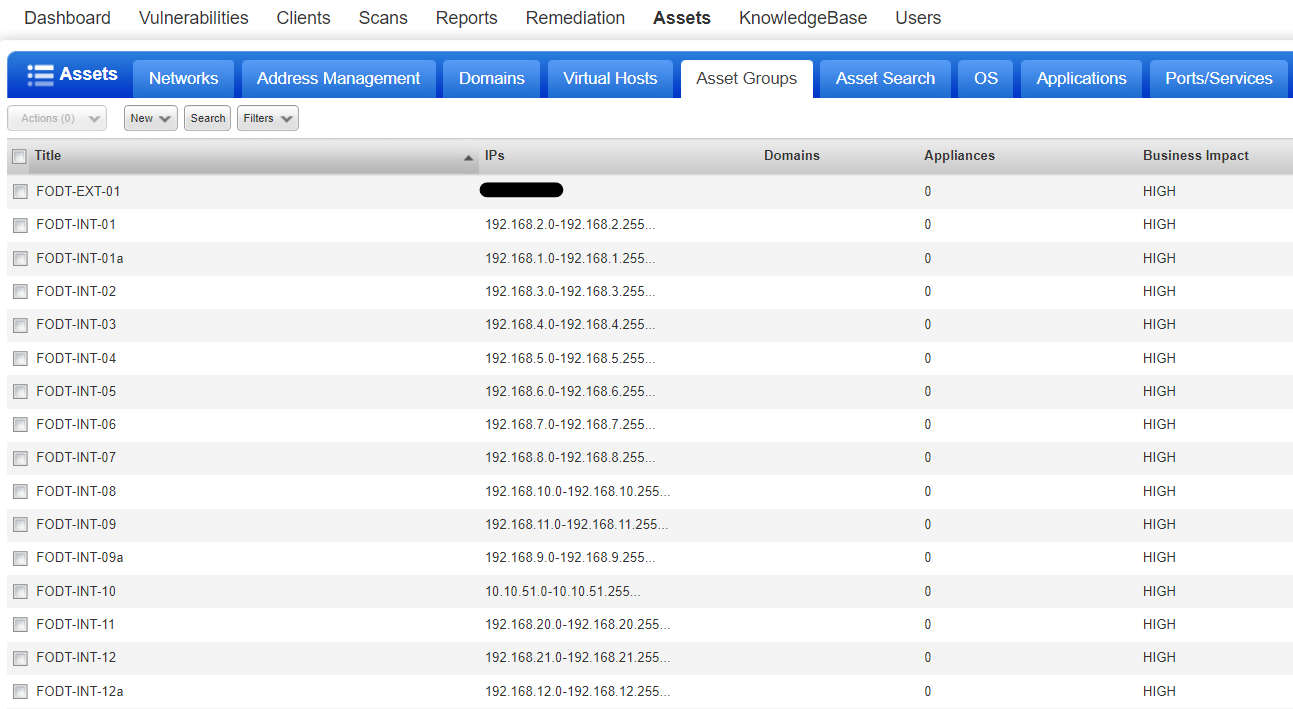
\includegraphics[width=1\linewidth]{images/qualys_targets.png}
    \caption{: Lista degli \textit{asset groups}. Ogni gruppo è costituito da indirizzi IP singoli, intervalli o \textit{subnet} intere, o da specifici nomi di dominio.}
    \label{fig:qualys_targets}
\end{figure}

\begin{figure}
\centering
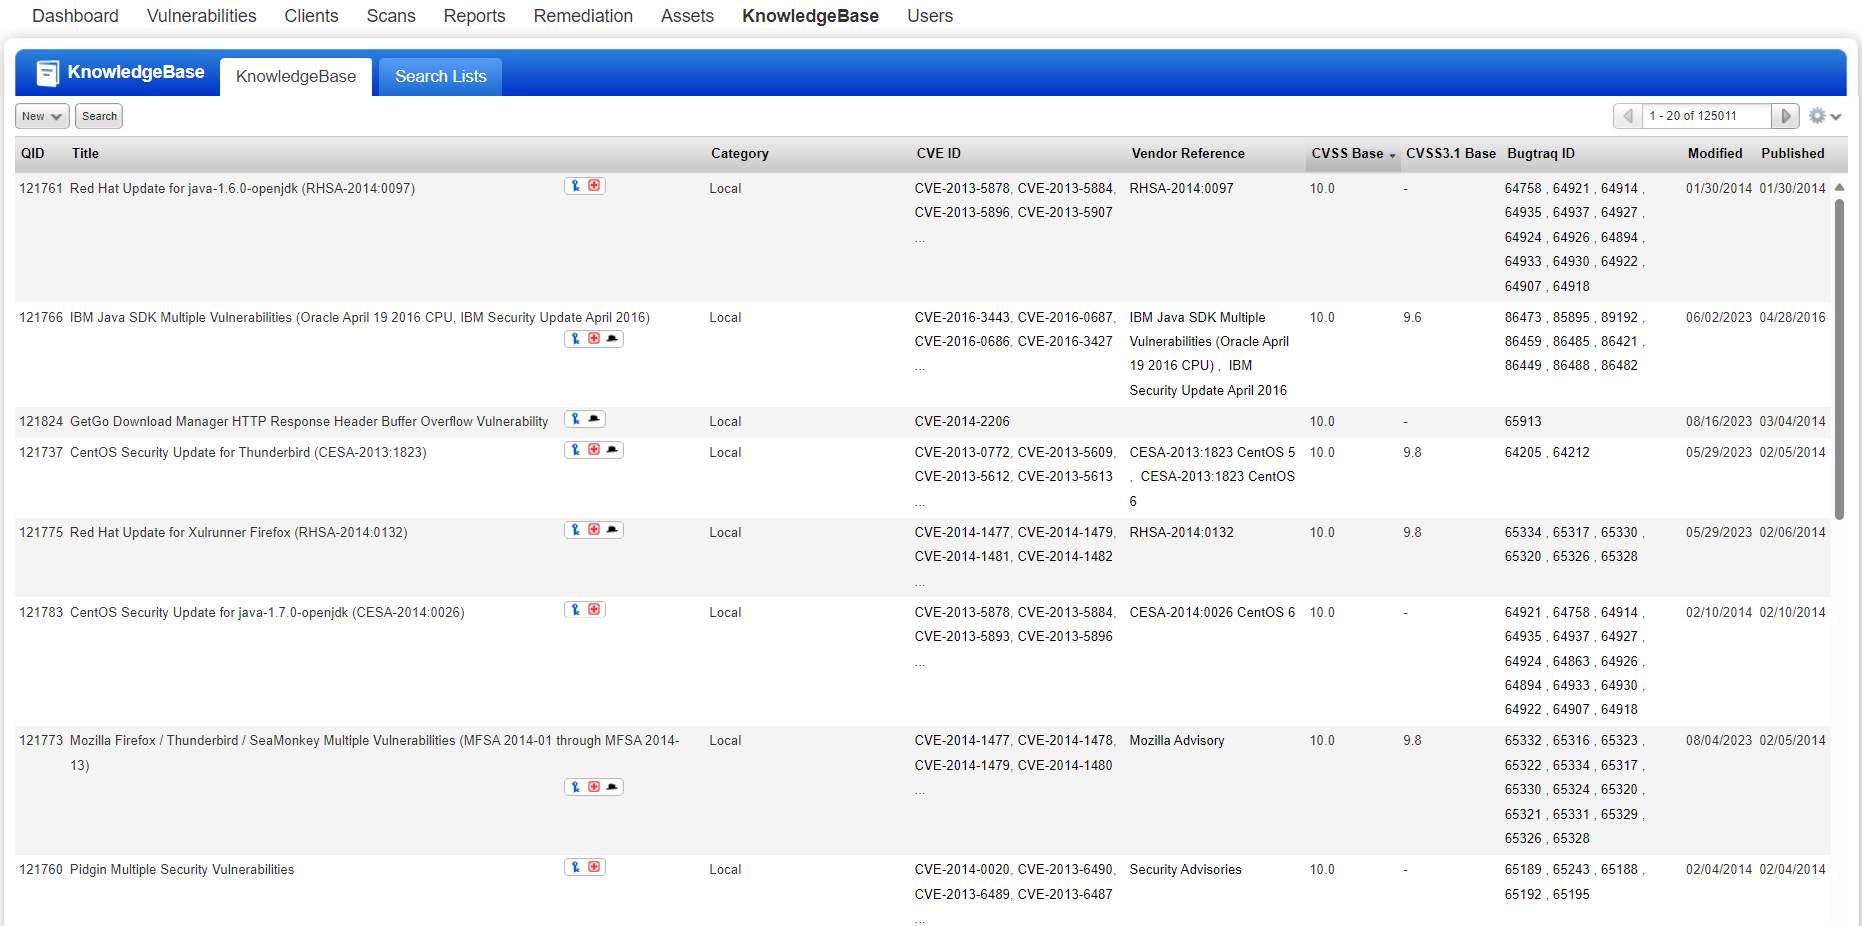
\includegraphics[scale=0.35]{images/qualys_kb.png}
    \caption{: \textit{Knowledgebase}. Questo è il database delle vulnerabilità proprietario di \textit{Qualys} costantemente aggiornato. È possibile, per ogni voce, aggiungere commenti che verranno visualizzati nei report, modificare il livello di criticità delle vulnerabilità o disabilitarle in modo che le scansioni le ignorino.}
\end{figure}


%% Parte conclusiva del documento; tipicamente per riassunto, bibliografia e/o indice analitico.
\backmatter

%% Bibliografia (praticamente obbligatoria)


\bibliographystyle{plain}%% Carica l'omonimo file .bst, dove \languagename è la lingua attiva.
%% Nel caso in cui si usi un file .bib (consigliato)
\bibliography{thud.bib}
%% Nel caso di bibliografia manuale, usare l'environment thebibliography.

%% Per l'indice analitico, usare il pacchetto makeidx (o analogo).

\end{document}
